\documentclass{article} % For LaTeX2e
\usepackage{iclr2025_conference,times}

% Optional math commands from https://github.com/goodfeli/dlbook_notation.
%%%%% NEW MATH DEFINITIONS %%%%%

\usepackage{amsmath,amsfonts,bm}

% Mark sections of captions for referring to divisions of figures
\newcommand{\figleft}{{\em (Left)}}
\newcommand{\figcenter}{{\em (Center)}}
\newcommand{\figright}{{\em (Right)}}
\newcommand{\figtop}{{\em (Top)}}
\newcommand{\figbottom}{{\em (Bottom)}}
\newcommand{\captiona}{{\em (a)}}
\newcommand{\captionb}{{\em (b)}}
\newcommand{\captionc}{{\em (c)}}
\newcommand{\captiond}{{\em (d)}}

% Highlight a newly defined term
\newcommand{\newterm}[1]{{\bf #1}}


% Figure reference, lower-case.
\def\figref#1{figure~\ref{#1}}
% Figure reference, capital. For start of sentence
\def\Figref#1{Figure~\ref{#1}}
\def\twofigref#1#2{figures \ref{#1} and \ref{#2}}
\def\quadfigref#1#2#3#4{figures \ref{#1}, \ref{#2}, \ref{#3} and \ref{#4}}
% Section reference, lower-case.
\def\secref#1{section~\ref{#1}}
% Section reference, capital.
\def\Secref#1{Section~\ref{#1}}
% Reference to two sections.
\def\twosecrefs#1#2{sections \ref{#1} and \ref{#2}}
% Reference to three sections.
\def\secrefs#1#2#3{sections \ref{#1}, \ref{#2} and \ref{#3}}
% Reference to an equation, lower-case.
\def\eqref#1{equation~\ref{#1}}
% Reference to an equation, upper case
\def\Eqref#1{Equation~\ref{#1}}
% A raw reference to an equation---avoid using if possible
\def\plaineqref#1{\ref{#1}}
% Reference to a chapter, lower-case.
\def\chapref#1{chapter~\ref{#1}}
% Reference to an equation, upper case.
\def\Chapref#1{Chapter~\ref{#1}}
% Reference to a range of chapters
\def\rangechapref#1#2{chapters\ref{#1}--\ref{#2}}
% Reference to an algorithm, lower-case.
\def\algref#1{algorithm~\ref{#1}}
% Reference to an algorithm, upper case.
\def\Algref#1{Algorithm~\ref{#1}}
\def\twoalgref#1#2{algorithms \ref{#1} and \ref{#2}}
\def\Twoalgref#1#2{Algorithms \ref{#1} and \ref{#2}}
% Reference to a part, lower case
\def\partref#1{part~\ref{#1}}
% Reference to a part, upper case
\def\Partref#1{Part~\ref{#1}}
\def\twopartref#1#2{parts \ref{#1} and \ref{#2}}

\def\ceil#1{\lceil #1 \rceil}
\def\floor#1{\lfloor #1 \rfloor}
\def\1{\bm{1}}
\newcommand{\train}{\mathcal{D}}
\newcommand{\valid}{\mathcal{D_{\mathrm{valid}}}}
\newcommand{\test}{\mathcal{D_{\mathrm{test}}}}

\def\eps{{\epsilon}}


% Random variables
\def\reta{{\textnormal{$\eta$}}}
\def\ra{{\textnormal{a}}}
\def\rb{{\textnormal{b}}}
\def\rc{{\textnormal{c}}}
\def\rd{{\textnormal{d}}}
\def\re{{\textnormal{e}}}
\def\rf{{\textnormal{f}}}
\def\rg{{\textnormal{g}}}
\def\rh{{\textnormal{h}}}
\def\ri{{\textnormal{i}}}
\def\rj{{\textnormal{j}}}
\def\rk{{\textnormal{k}}}
\def\rl{{\textnormal{l}}}
% rm is already a command, just don't name any random variables m
\def\rn{{\textnormal{n}}}
\def\ro{{\textnormal{o}}}
\def\rp{{\textnormal{p}}}
\def\rq{{\textnormal{q}}}
\def\rr{{\textnormal{r}}}
\def\rs{{\textnormal{s}}}
\def\rt{{\textnormal{t}}}
\def\ru{{\textnormal{u}}}
\def\rv{{\textnormal{v}}}
\def\rw{{\textnormal{w}}}
\def\rx{{\textnormal{x}}}
\def\ry{{\textnormal{y}}}
\def\rz{{\textnormal{z}}}

% Random vectors
\def\rvepsilon{{\mathbf{\epsilon}}}
\def\rvtheta{{\mathbf{\theta}}}
\def\rva{{\mathbf{a}}}
\def\rvb{{\mathbf{b}}}
\def\rvc{{\mathbf{c}}}
\def\rvd{{\mathbf{d}}}
\def\rve{{\mathbf{e}}}
\def\rvf{{\mathbf{f}}}
\def\rvg{{\mathbf{g}}}
\def\rvh{{\mathbf{h}}}
\def\rvu{{\mathbf{i}}}
\def\rvj{{\mathbf{j}}}
\def\rvk{{\mathbf{k}}}
\def\rvl{{\mathbf{l}}}
\def\rvm{{\mathbf{m}}}
\def\rvn{{\mathbf{n}}}
\def\rvo{{\mathbf{o}}}
\def\rvp{{\mathbf{p}}}
\def\rvq{{\mathbf{q}}}
\def\rvr{{\mathbf{r}}}
\def\rvs{{\mathbf{s}}}
\def\rvt{{\mathbf{t}}}
\def\rvu{{\mathbf{u}}}
\def\rvv{{\mathbf{v}}}
\def\rvw{{\mathbf{w}}}
\def\rvx{{\mathbf{x}}}
\def\rvy{{\mathbf{y}}}
\def\rvz{{\mathbf{z}}}

% Elements of random vectors
\def\erva{{\textnormal{a}}}
\def\ervb{{\textnormal{b}}}
\def\ervc{{\textnormal{c}}}
\def\ervd{{\textnormal{d}}}
\def\erve{{\textnormal{e}}}
\def\ervf{{\textnormal{f}}}
\def\ervg{{\textnormal{g}}}
\def\ervh{{\textnormal{h}}}
\def\ervi{{\textnormal{i}}}
\def\ervj{{\textnormal{j}}}
\def\ervk{{\textnormal{k}}}
\def\ervl{{\textnormal{l}}}
\def\ervm{{\textnormal{m}}}
\def\ervn{{\textnormal{n}}}
\def\ervo{{\textnormal{o}}}
\def\ervp{{\textnormal{p}}}
\def\ervq{{\textnormal{q}}}
\def\ervr{{\textnormal{r}}}
\def\ervs{{\textnormal{s}}}
\def\ervt{{\textnormal{t}}}
\def\ervu{{\textnormal{u}}}
\def\ervv{{\textnormal{v}}}
\def\ervw{{\textnormal{w}}}
\def\ervx{{\textnormal{x}}}
\def\ervy{{\textnormal{y}}}
\def\ervz{{\textnormal{z}}}

% Random matrices
\def\rmA{{\mathbf{A}}}
\def\rmB{{\mathbf{B}}}
\def\rmC{{\mathbf{C}}}
\def\rmD{{\mathbf{D}}}
\def\rmE{{\mathbf{E}}}
\def\rmF{{\mathbf{F}}}
\def\rmG{{\mathbf{G}}}
\def\rmH{{\mathbf{H}}}
\def\rmI{{\mathbf{I}}}
\def\rmJ{{\mathbf{J}}}
\def\rmK{{\mathbf{K}}}
\def\rmL{{\mathbf{L}}}
\def\rmM{{\mathbf{M}}}
\def\rmN{{\mathbf{N}}}
\def\rmO{{\mathbf{O}}}
\def\rmP{{\mathbf{P}}}
\def\rmQ{{\mathbf{Q}}}
\def\rmR{{\mathbf{R}}}
\def\rmS{{\mathbf{S}}}
\def\rmT{{\mathbf{T}}}
\def\rmU{{\mathbf{U}}}
\def\rmV{{\mathbf{V}}}
\def\rmW{{\mathbf{W}}}
\def\rmX{{\mathbf{X}}}
\def\rmY{{\mathbf{Y}}}
\def\rmZ{{\mathbf{Z}}}

% Elements of random matrices
\def\ermA{{\textnormal{A}}}
\def\ermB{{\textnormal{B}}}
\def\ermC{{\textnormal{C}}}
\def\ermD{{\textnormal{D}}}
\def\ermE{{\textnormal{E}}}
\def\ermF{{\textnormal{F}}}
\def\ermG{{\textnormal{G}}}
\def\ermH{{\textnormal{H}}}
\def\ermI{{\textnormal{I}}}
\def\ermJ{{\textnormal{J}}}
\def\ermK{{\textnormal{K}}}
\def\ermL{{\textnormal{L}}}
\def\ermM{{\textnormal{M}}}
\def\ermN{{\textnormal{N}}}
\def\ermO{{\textnormal{O}}}
\def\ermP{{\textnormal{P}}}
\def\ermQ{{\textnormal{Q}}}
\def\ermR{{\textnormal{R}}}
\def\ermS{{\textnormal{S}}}
\def\ermT{{\textnormal{T}}}
\def\ermU{{\textnormal{U}}}
\def\ermV{{\textnormal{V}}}
\def\ermW{{\textnormal{W}}}
\def\ermX{{\textnormal{X}}}
\def\ermY{{\textnormal{Y}}}
\def\ermZ{{\textnormal{Z}}}

% Vectors
\def\vzero{{\bm{0}}}
\def\vone{{\bm{1}}}
\def\vmu{{\bm{\mu}}}
\def\vtheta{{\bm{\theta}}}
\def\va{{\bm{a}}}
\def\vb{{\bm{b}}}
\def\vc{{\bm{c}}}
\def\vd{{\bm{d}}}
\def\ve{{\bm{e}}}
\def\vf{{\bm{f}}}
\def\vg{{\bm{g}}}
\def\vh{{\bm{h}}}
\def\vi{{\bm{i}}}
\def\vj{{\bm{j}}}
\def\vk{{\bm{k}}}
\def\vl{{\bm{l}}}
\def\vm{{\bm{m}}}
\def\vn{{\bm{n}}}
\def\vo{{\bm{o}}}
\def\vp{{\bm{p}}}
\def\vq{{\bm{q}}}
\def\vr{{\bm{r}}}
\def\vs{{\bm{s}}}
\def\vt{{\bm{t}}}
\def\vu{{\bm{u}}}
\def\vv{{\bm{v}}}
\def\vw{{\bm{w}}}
\def\vx{{\bm{x}}}
\def\vy{{\bm{y}}}
\def\vz{{\bm{z}}}

% Elements of vectors
\def\evalpha{{\alpha}}
\def\evbeta{{\beta}}
\def\evepsilon{{\epsilon}}
\def\evlambda{{\lambda}}
\def\evomega{{\omega}}
\def\evmu{{\mu}}
\def\evpsi{{\psi}}
\def\evsigma{{\sigma}}
\def\evtheta{{\theta}}
\def\eva{{a}}
\def\evb{{b}}
\def\evc{{c}}
\def\evd{{d}}
\def\eve{{e}}
\def\evf{{f}}
\def\evg{{g}}
\def\evh{{h}}
\def\evi{{i}}
\def\evj{{j}}
\def\evk{{k}}
\def\evl{{l}}
\def\evm{{m}}
\def\evn{{n}}
\def\evo{{o}}
\def\evp{{p}}
\def\evq{{q}}
\def\evr{{r}}
\def\evs{{s}}
\def\evt{{t}}
\def\evu{{u}}
\def\evv{{v}}
\def\evw{{w}}
\def\evx{{x}}
\def\evy{{y}}
\def\evz{{z}}

% Matrix
\def\mA{{\bm{A}}}
\def\mB{{\bm{B}}}
\def\mC{{\bm{C}}}
\def\mD{{\bm{D}}}
\def\mE{{\bm{E}}}
\def\mF{{\bm{F}}}
\def\mG{{\bm{G}}}
\def\mH{{\bm{H}}}
\def\mI{{\bm{I}}}
\def\mJ{{\bm{J}}}
\def\mK{{\bm{K}}}
\def\mL{{\bm{L}}}
\def\mM{{\bm{M}}}
\def\mN{{\bm{N}}}
\def\mO{{\bm{O}}}
\def\mP{{\bm{P}}}
\def\mQ{{\bm{Q}}}
\def\mR{{\bm{R}}}
\def\mS{{\bm{S}}}
\def\mT{{\bm{T}}}
\def\mU{{\bm{U}}}
\def\mV{{\bm{V}}}
\def\mW{{\bm{W}}}
\def\mX{{\bm{X}}}
\def\mY{{\bm{Y}}}
\def\mZ{{\bm{Z}}}
\def\mBeta{{\bm{\beta}}}
\def\mPhi{{\bm{\Phi}}}
\def\mLambda{{\bm{\Lambda}}}
\def\mSigma{{\bm{\Sigma}}}

% Tensor
\DeclareMathAlphabet{\mathsfit}{\encodingdefault}{\sfdefault}{m}{sl}
\SetMathAlphabet{\mathsfit}{bold}{\encodingdefault}{\sfdefault}{bx}{n}
\newcommand{\tens}[1]{\bm{\mathsfit{#1}}}
\def\tA{{\tens{A}}}
\def\tB{{\tens{B}}}
\def\tC{{\tens{C}}}
\def\tD{{\tens{D}}}
\def\tE{{\tens{E}}}
\def\tF{{\tens{F}}}
\def\tG{{\tens{G}}}
\def\tH{{\tens{H}}}
\def\tI{{\tens{I}}}
\def\tJ{{\tens{J}}}
\def\tK{{\tens{K}}}
\def\tL{{\tens{L}}}
\def\tM{{\tens{M}}}
\def\tN{{\tens{N}}}
\def\tO{{\tens{O}}}
\def\tP{{\tens{P}}}
\def\tQ{{\tens{Q}}}
\def\tR{{\tens{R}}}
\def\tS{{\tens{S}}}
\def\tT{{\tens{T}}}
\def\tU{{\tens{U}}}
\def\tV{{\tens{V}}}
\def\tW{{\tens{W}}}
\def\tX{{\tens{X}}}
\def\tY{{\tens{Y}}}
\def\tZ{{\tens{Z}}}


% Graph
\def\gA{{\mathcal{A}}}
\def\gB{{\mathcal{B}}}
\def\gC{{\mathcal{C}}}
\def\gD{{\mathcal{D}}}
\def\gE{{\mathcal{E}}}
\def\gF{{\mathcal{F}}}
\def\gG{{\mathcal{G}}}
\def\gH{{\mathcal{H}}}
\def\gI{{\mathcal{I}}}
\def\gJ{{\mathcal{J}}}
\def\gK{{\mathcal{K}}}
\def\gL{{\mathcal{L}}}
\def\gM{{\mathcal{M}}}
\def\gN{{\mathcal{N}}}
\def\gO{{\mathcal{O}}}
\def\gP{{\mathcal{P}}}
\def\gQ{{\mathcal{Q}}}
\def\gR{{\mathcal{R}}}
\def\gS{{\mathcal{S}}}
\def\gT{{\mathcal{T}}}
\def\gU{{\mathcal{U}}}
\def\gV{{\mathcal{V}}}
\def\gW{{\mathcal{W}}}
\def\gX{{\mathcal{X}}}
\def\gY{{\mathcal{Y}}}
\def\gZ{{\mathcal{Z}}}

% Sets
\def\sA{{\mathbb{A}}}
\def\sB{{\mathbb{B}}}
\def\sC{{\mathbb{C}}}
\def\sD{{\mathbb{D}}}
% Don't use a set called E, because this would be the same as our symbol
% for expectation.
\def\sF{{\mathbb{F}}}
\def\sG{{\mathbb{G}}}
\def\sH{{\mathbb{H}}}
\def\sI{{\mathbb{I}}}
\def\sJ{{\mathbb{J}}}
\def\sK{{\mathbb{K}}}
\def\sL{{\mathbb{L}}}
\def\sM{{\mathbb{M}}}
\def\sN{{\mathbb{N}}}
\def\sO{{\mathbb{O}}}
\def\sP{{\mathbb{P}}}
\def\sQ{{\mathbb{Q}}}
\def\sR{{\mathbb{R}}}
\def\sS{{\mathbb{S}}}
\def\sT{{\mathbb{T}}}
\def\sU{{\mathbb{U}}}
\def\sV{{\mathbb{V}}}
\def\sW{{\mathbb{W}}}
\def\sX{{\mathbb{X}}}
\def\sY{{\mathbb{Y}}}
\def\sZ{{\mathbb{Z}}}

% Entries of a matrix
\def\emLambda{{\Lambda}}
\def\emA{{A}}
\def\emB{{B}}
\def\emC{{C}}
\def\emD{{D}}
\def\emE{{E}}
\def\emF{{F}}
\def\emG{{G}}
\def\emH{{H}}
\def\emI{{I}}
\def\emJ{{J}}
\def\emK{{K}}
\def\emL{{L}}
\def\emM{{M}}
\def\emN{{N}}
\def\emO{{O}}
\def\emP{{P}}
\def\emQ{{Q}}
\def\emR{{R}}
\def\emS{{S}}
\def\emT{{T}}
\def\emU{{U}}
\def\emV{{V}}
\def\emW{{W}}
\def\emX{{X}}
\def\emY{{Y}}
\def\emZ{{Z}}
\def\emSigma{{\Sigma}}

% entries of a tensor
% Same font as tensor, without \bm wrapper
\newcommand{\etens}[1]{\mathsfit{#1}}
\def\etLambda{{\etens{\Lambda}}}
\def\etA{{\etens{A}}}
\def\etB{{\etens{B}}}
\def\etC{{\etens{C}}}
\def\etD{{\etens{D}}}
\def\etE{{\etens{E}}}
\def\etF{{\etens{F}}}
\def\etG{{\etens{G}}}
\def\etH{{\etens{H}}}
\def\etI{{\etens{I}}}
\def\etJ{{\etens{J}}}
\def\etK{{\etens{K}}}
\def\etL{{\etens{L}}}
\def\etM{{\etens{M}}}
\def\etN{{\etens{N}}}
\def\etO{{\etens{O}}}
\def\etP{{\etens{P}}}
\def\etQ{{\etens{Q}}}
\def\etR{{\etens{R}}}
\def\etS{{\etens{S}}}
\def\etT{{\etens{T}}}
\def\etU{{\etens{U}}}
\def\etV{{\etens{V}}}
\def\etW{{\etens{W}}}
\def\etX{{\etens{X}}}
\def\etY{{\etens{Y}}}
\def\etZ{{\etens{Z}}}

% The true underlying data generating distribution
\newcommand{\pdata}{p_{\rm{data}}}
% The empirical distribution defined by the training set
\newcommand{\ptrain}{\hat{p}_{\rm{data}}}
\newcommand{\Ptrain}{\hat{P}_{\rm{data}}}
% The model distribution
\newcommand{\pmodel}{p_{\rm{model}}}
\newcommand{\Pmodel}{P_{\rm{model}}}
\newcommand{\ptildemodel}{\tilde{p}_{\rm{model}}}
% Stochastic autoencoder distributions
\newcommand{\pencode}{p_{\rm{encoder}}}
\newcommand{\pdecode}{p_{\rm{decoder}}}
\newcommand{\precons}{p_{\rm{reconstruct}}}

\newcommand{\laplace}{\mathrm{Laplace}} % Laplace distribution

\newcommand{\E}{\mathbb{E}}
\newcommand{\Ls}{\mathcal{L}}
\newcommand{\R}{\mathbb{R}}
\newcommand{\emp}{\tilde{p}}
\newcommand{\lr}{\alpha}
\newcommand{\reg}{\lambda}
\newcommand{\rect}{\mathrm{rectifier}}
\newcommand{\softmax}{\mathrm{softmax}}
\newcommand{\sigmoid}{\sigma}
\newcommand{\softplus}{\zeta}
\newcommand{\KL}{D_{\mathrm{KL}}}
\newcommand{\Var}{\mathrm{Var}}
\newcommand{\standarderror}{\mathrm{SE}}
\newcommand{\Cov}{\mathrm{Cov}}
% Wolfram Mathworld says $L^2$ is for function spaces and $\ell^2$ is for vectors
% But then they seem to use $L^2$ for vectors throughout the site, and so does
% wikipedia.
\newcommand{\normlzero}{L^0}
\newcommand{\normlone}{L^1}
\newcommand{\normltwo}{L^2}
\newcommand{\normlp}{L^p}
\newcommand{\normmax}{L^\infty}

\newcommand{\parents}{Pa} % See usage in notation.tex. Chosen to match Daphne's book.

\DeclareMathOperator*{\argmax}{arg\,max}
\DeclareMathOperator*{\argmin}{arg\,min}

\DeclareMathOperator{\sign}{sign}
\DeclareMathOperator{\Tr}{Tr}
\let\ab\allowbreak


\usepackage{hyperref}
\usepackage{url}
\usepackage{graphicx}
\usepackage{booktabs}
\usepackage{tabularx}
\usepackage{array}
\usepackage{placeins}

%%%%%%%%% TITLE - PLEASE UPDATE TITLE HERE
\title{Holding the Sources Fixed: A Controlled Benchmark of Strategies for Writing Curated Genetics Knowledge-Base Entries from Cited Papers}

\author{Ambitious AI Researcher\\
AI Research Institute\\
123 AI Avenue, ML City\\
\texttt{researcher@institute.ai}
}

\newcommand{\fix}{\marginpar{FIX}}
\newcommand{\new}{\marginpar{NEW}}
\newcommand{\pp}[1]{$#1$}

\begin{document}

\maketitle


\begin{abstract}
%%%%%%%%% ABSTRACT %%%%%%%%%
Comparisons of long-context reading, retrieval and intermediate representations exist, but on question answering, summarisation or open retrieval scored against benchmark answers. We build a controlled benchmark for the curator's own task, writing a whole knowledge-base entry, in which the generation strategy is the only variable: each of 100 OMIM phenotype entries with 2--12 references is written from exactly the papers its curators cited, causal gene withheld, by one model under the same guards, claim-level audit and scoring. Three paradigms (read and write; extract, then write; memory first), a memory-only control and three add-ons are scored on coverage of fixed fact lists from curator-written per-paper text (OMIM facts conveyed). Because curators wrote from full papers, less text must convey less; we measure how much within the same papers: hiding their full text lowers coverage from 77.4\% to 31.2\% (46 entries; paired difference $+43.9$ points, 95\% interval $+38.5$ to $+49.3$), many times any difference between reading strategies. In the regime tested (19\% of papers readable in full, inputs that fit one prompt, one model), the reading strategies are close on the 93 entries every strategy completed (47.2--49.1\%; replicate-noise half-width 1.0 point), memory-first strategies convey 15.1\% and 14.6\%, and the strategies separate where more full text is readable. Measurement choices matter at this resolution: treating stopped replies asymmetrically produced a spurious 2.1-point deficit. The audit flagged all 60 planted single-fact errors, but its false-flag rate was not measured and it checks fidelity to the cited text, not correctness. One model family wrote, audited and judged everything, and no human validated any judgement.
%%%%%%%%% ABSTRACT %%%%%%%%%
\end{abstract}

\section{Introduction}
\label{sec:intro}
%%%%%%%%% INTRODUCTION %%%%%%%%%
Curated knowledge bases are written by experts who read papers and record, entry by entry, what each paper showed. Online Mendelian Inheritance in Man (OMIM), the reference catalogue of human genes and genetic disorders \citep{Amberger2014OmimorgOnline,amberger2019omim,hamosh2021online}, is built this way, and so, in part, are the resources that record variant interpretations \citep{Landrum2017ClinvarImproving,landrum2025clinvar}, phenotype annotations \citep{robinson2008human,gargano2024human} and the validity of gene--disease associations \citep{strande2017evaluating}. Automated text mining already annotates biomedical concepts across PubMed abstracts and open-access full text \citep{Wei2019PubtatorCentral,wei2024pubtator}, variants can be searched across full text and supplementary data \citep{allot2023tracking}, and language models can now read the papers themselves. Many system designs have been proposed for turning a set of documents into structured, cited text: retrieval-augmented or long-context reading \citep{Lewis2020RetrievalaugmentedGeneration,li2024retrieval}, extraction into a graph or a table before writing \citep{edge2024local,joshi2026sliders}, agents that decide what to read \citep{Nakano2021WebgptBrowserassisted,Lla2023PaperqaRetrievalaugmented,skarlinski2024language}, drafting first and verifying afterwards \citep{Gao2022RarrResearching,dhuliawala2024chainofverification}, and prompts optimised from examples \citep{Khattab2023DspyCompiling,agrawal2026gepa}. Reviews assess such tools for evidence synthesis \citep{Clark2025GenerativeArtificial,scherbakov2025emergence}, and language-model workflows now automate screening and data extraction for systematic reviews \citep{cao2025automation,wang2025accelerating}.

Comparisons between such designs exist, and several hold the model and settings fixed \citep{li2024retrieval,Li2025LaraBenchmarking,han2025rag}; they concern question answering, summarisation or open retrieval scored against benchmark answers. The closest work in genetics and biology searches a corpus for its sources, measures memory alone, or scores against something other than what curators wrote about each paper (Section~\ref{sec:related_work}; \citealp{zhang2026flyaoc,yan2026genknowrd,skarlinski2024language,groza2026systematic}). The curator's task itself, writing a whole entry from exactly the papers the curators cited and scored against what they wrote, has not been used to compare strategies. Three questions are open. With the model, the sources, the guards and the scoring held fixed, how much does the generation strategy matter? What limits agreement with what experts wrote: the strategy, or what the strategy was given to read? And which errors does a claim-level audit against the cited source catch, and which can it not see?

We answer them with a controlled benchmark in which the generation strategy is the only variable (Figure~\ref{fig:overview}). Each of 100 OMIM phenotype entries with 2--12 references is written from its header and exactly the papers its curators cited, with the causal gene withheld; only 19\% of the cited papers are readable in full through open access. One model writes every draft under the same guards, audit and scoring. The strategies form three paradigms (\emph{read and write}; \emph{extract, then write}; \emph{memory first}), one control (a memory-only draft with no papers) and three add-ons, each tested against its parent, and access to each source is itself measured and manipulated. The primary endpoint is \emph{OMIM facts conveyed}: coverage of the facts in OMIM's allelic-variant descriptions as deposited in ClinVar, curator-written, variant-centred paragraphs about individual cited papers, each split once, without sight of any draft, into a fixed list of facts (6,652 in all over 476 paragraphs) reused for every strategy.

\textbf{In the regime tested, access to the source bounds agreement with curators far more than the reading strategy does.} Curators wrote from full papers, so drafts written from less text must convey less; we measure how much within the same papers and attribute every missed fact to text the model read or did not read. When the full text of papers that have one is hidden and the same entries are rewritten from their abstracts, coverage of the same fixed facts falls from 77.4\% to 31.2\% (paired difference $+43.9$ points, $+38.5$ to $+49.3$). At current open access this is many times any difference between reading strategies: on the 93 entries every strategy completed, only the case table's difference from direct reading ($-1.9$, $-3.1$ to $-0.8$) exceeds the replicate-noise half-width of 1.0 point. This closeness is shown for entries with 2--12 references, inputs that fit one prompt and one model; where more full text is readable the strategies separate, and in a matched ablation the gap of our extract-then-write implementations depends on extraction effort.

Our contributions are: (1) a benchmark and harness for evidence-grounded knowledge-base writing against curator-written references, built only from public resources \citep{sayers2026database,Louden2020MedgenNcbis,rosonovski2024europe,seal2023genenames}, with a claim-level audit, fixed fact lists and per-entry release of every draft, verdict and score; (2) a controlled comparison of three paradigms, a control and three add-ons under one model that reports completion (replies stopped by the model's safety filter are an outcome, not an exclusion), variance between repeated runs and matched ablations; (3) a within-paper measurement of how much access to the source bounds agreement with curators, with every missed fact attributed to text the model read or did not read; (4) a characterisation of what the audit can and cannot see; (5) a memory-only control by creation date as a contamination check, with negative results, at this scale, for recall-then-verify, a small learned guide and reconciliation; and (6) measurement lessons for comparing such systems (Section~\ref{sec:discussion}): an asymmetric completion rule produced a spurious 2.1-point deficit, per-draft fact splitting changes levels, run-to-run noise is as large as the differences between reading strategies, and a pipeline's apparent deficit depended on a setting unrelated to its representation. The study is scoped to what was run: one model family wrote, audited and judged everything; no curator has read any draft, verdict or fact judgement; only open-access text without supplementary material was available; every strategy was given the curators' reference list; and the strategies were developed on the evaluation entries. The generated entries are drafts for expert review, not clinical guidance.
%%%%%%%%% INTRODUCTION %%%%%%%%%

\section{Related Work}
\label{sec:related_work}
%%%%%%%%% RELATED WORK %%%%%%%%%
We organise prior work along the axes our strategies vary. Published systems were not run here; the strategies we compare are our own implementations of the ideas below.

\paragraph{Language models for literature curation in genetics and biology.}
Concept recognition against the Human Phenotype Ontology uses dedicated taggers \citep{luo2021phenotagger,groza2024fasthpocr} and, increasingly, language models \citep{groza2024evaluation,yang2024enhancing,garcia2025improving}. For populating and maintaining knowledge bases, structured prompting and assistant tools have been proposed \citep{caufield2024structured,caufield2024curategpt,toro2024dynamic,niyonkuru2025leveraging}, as have an agent that assists manual gene function annotation \citep{Li2025GenewhispererEnhancing}, generative annotation of the severity of ontology phenotypes \citep{Murphy2024HarnessingGenerative}, and agents for ontology curation of natural phenotypes \citep{balhoff2026frontier}. Closer to clinical genetics, language models have been applied to extracting variant, gene--disease and gene--phenotype evidence from papers \citep{li2025autopm3,furlan2025eagleai,wang2026pubmind,yin2026benchmarking}, benchmarked on clinical-genetics reasoning \citep{queen2025cgbench}, given database tools for genomics questions \citep{Jin2023GenegptAugmenting}, and evaluated for gene-set function \citep{hu2025evaluation}, gene prioritisation \citep{Kim2024AssessingUtility} and rare-disease diagnostics \citep{twede2026evidence}. The four closest studies differ from ours in what is held fixed and what serves as the reference. FlyAOC scores memorisation, pipeline and agent harnesses that search a paper corpus against FlyBase curators' annotations \citep{zhang2026flyaoc}; GEN-KnowRD generates schema-guided rare-disease profiles, assesses their quality and builds a knowledge base from them, evaluated by disease ranking on patient benchmarks \citep{yan2026genknowrd}; PaperQA2 writes cited Wikipedia-style summaries of scientific topics, compared against existing Wikipedia articles \citep{skarlinski2024language}; and \citet{groza2026systematic} measure model memory of rare-disease genes and phenotypes. In our benchmark the cited papers are fixed, the reference is the curators' own per-paper text and structured fields, and the generation strategy is the only variable.

\paragraph{Intermediate representations versus long-context reading.}
Retrieval augmentation supplies a model with selected passages \citep{Lewis2020RetrievalaugmentedGeneration}, possibly retrieving on demand and critiquing its own output \citep{Asai2023SelfragLearning}. Whether this beats placing all documents in a long context is contested: one re-evaluation finds long context generally ahead on question answering, especially for Wikipedia-based questions \citep{Li2024LongContext}; others argue that very long contexts dilute focus on relevant information \citep{Yu2024DefenseRag}, propose hybrids \citep{li2024retrieval}, or report no single winner \citep{Li2025LaraBenchmarking}. Graph intermediates are used for query-focused summarisation \citep{edge2024local} and retrieval inspired by hippocampal indexing \citep{Gutirrez2024HipporagNeurobiologically}, and systematic comparisons ask when graphs help \citep{han2025rag,xiang2025use}. Table- and database-centred pipelines rewrite document-processing operations agentically \citep{shankar2025docetl}, reconcile extracted databases for systematic reviews \citep{joshi2026sliders} or carry out deep research over large databases \citep{liu2026datastorm}. Agentic and retrieval-augmented systems write cited answers or articles from the scientific literature \citep{Lla2023PaperqaRetrievalaugmented,Asai2024OpenscholarSynthesizing,singh2025ai2,skarlinski2024language}, or Wikipedia-like articles from Internet sources \citep{shao2024assisting}. Several of these comparisons are controlled, holding the model fixed or standardising retrieval and generation settings \citep{li2024retrieval,Li2025LaraBenchmarking,han2025rag}, but on question answering, summarisation or open retrieval scored against benchmark answers. Here the task is writing a whole curated entry; the papers are fixed to the curators' reference list; the reference is the curators' own per-paper text and structured fields; read-and-write, extract-then-write and memory-first strategies and a memory-only control share one audit and one scoring; access to each source is measured and manipulated; and a matched ablation separates the intermediate representation from extraction effort.

\paragraph{Memory, verification and contamination.}
Draft-then-verify methods plan verification questions \citep{dhuliawala2024chainofverification}, post-edit unsupported content \citep{Gao2022RarrResearching}, use the consistency of sampled outputs \citep{Manakul2023SelfcheckgptZeroresource}, or check against domain databases \citep{wang2025geneagent}. Because curated knowledge bases are public, memory is also a confound. Surveys catalogue contamination, its detection and its mitigation \citep{Xu2024BenchmarkData,Deng2024UnveilingSpectrum,Ravaut2024ComprehensiveSurvey,Cheng2025SurveyData,Chen2025RecentAdvances}; methods detect pretraining data or contamination from black-box access \citep{Shi2023DetectingPretraining,oren2024proving,golchin2024time,Golchin2025DataContamination}, exploit training cut-offs as a natural experiment \citep{Roberts2023DataContamination}, or collect new test items over time \citep{Jain2024LivecodebenchHolistic,White2024LivebenchChallenging}. We adopt the time-based view within the task: a memory-only control analysed by entry creation date, and entries created in 2026.

\paragraph{Supervision by prompt optimisation.}
Instructions can be searched or optimised by language models \citep{Zhou2022LargeLanguage,Pryzant2023AutomaticPrompt,Yang2023LargeLanguage}, evolved \citep{Guo2023EvopromptConnecting,Fernando2023PromptbreederSelfreferential,agrawal2026gepa}, compiled with demonstrations in multi-stage programs \citep{Khattab2023DspyCompiling,Opsahlong2024OptimizingInstructions}, or updated from textual feedback \citep{Yuksekgonul2024TextgradAutomatic}. Our learned curation guide is a deliberately small instance of this idea; its result says nothing about better-resourced prompt optimisation.

\paragraph{Evaluating cited long-form text.}
Factuality metrics decompose long-form text into atomic claims and verify each against a knowledge source \citep{min2023factscore,wei2024longform}, and VeriScore restricts this to verifiable claims \citep{Song2024VeriscoreEvaluating}. Citation quality has been measured for models that generate text with citations \citep{gao2023enabling}, in human audits of generative search engines that check whether statements are supported by their citations \citep{Liu2023EvaluatingVerifiability}, and for medical references \citep{wu2025automated}; the accuracy with which medical articles quote their sources has itself been reviewed systematically \citep{jergas2015quotation}, which bears on our second-hand evidence. Work studies model judges against human preferences \citep{zheng2023judging,shankar2024who} and reports that evaluators recognise and favour their own generations \citep{panickssery2024llm}. Our audit and fact judgements use the same model family that wrote the drafts, with no human validation; we therefore report judge and replicate variation, fixed fact lists shared by all strategies and planted-error tests, and we describe audit verdicts as \emph{judged supported}. Text mining yields more from full text than from abstracts \citep{Westergaard2018ComprehensiveQuantitative}, whose structure and content differ \citep{Cohen2010StructuralContent}. That drafts written from abstracts convey less of what curators wrote from full papers is therefore expected; our access experiments measure how much, within the same papers, for knowledge-base writing.
%%%%%%%%% RELATED WORK %%%%%%%%%

\section{Benchmark and Strategies}
\label{sec:method}
%%%%%%%%% METHOD %%%%%%%%%
\begin{figure}[t]
\begin{center}
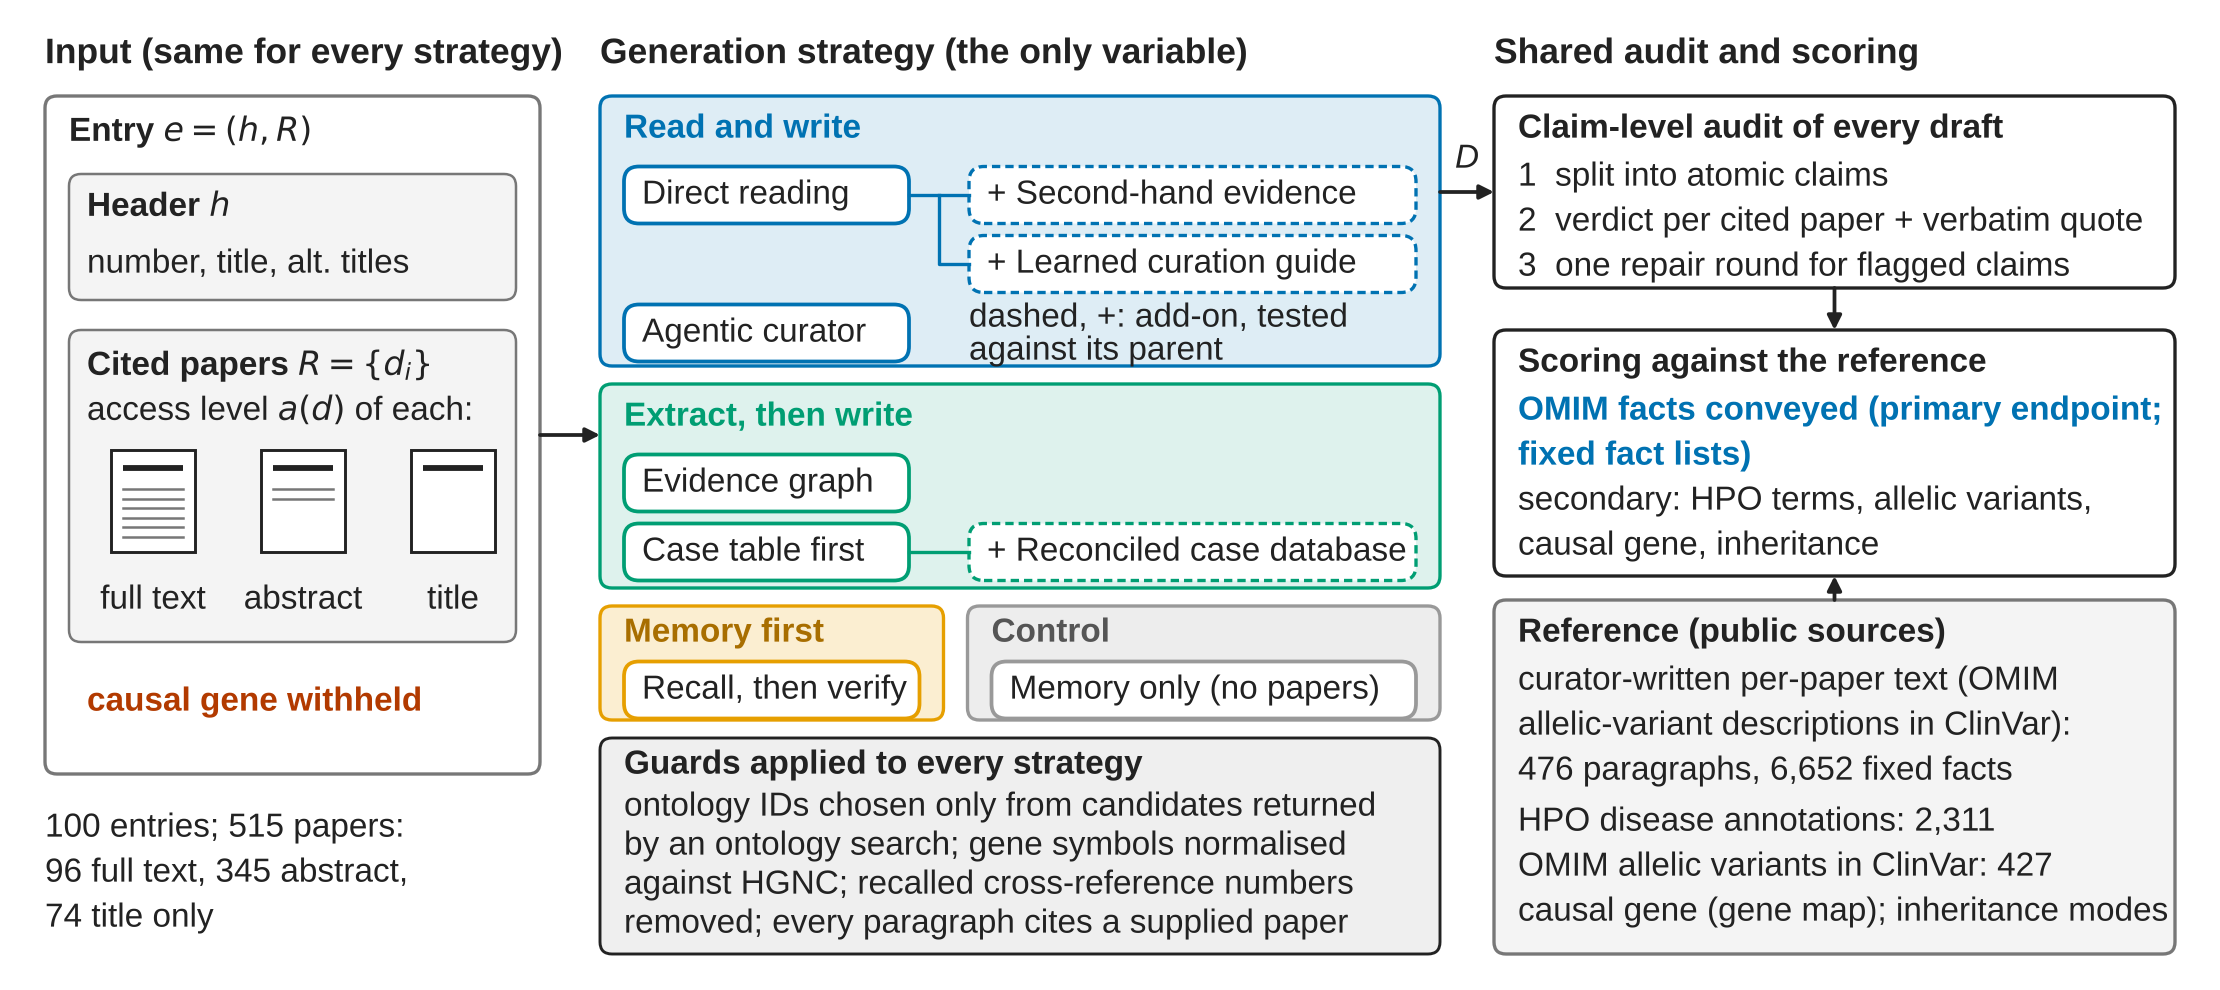
\includegraphics[width=0.86\linewidth]{figures/fig_benchmark_overview.png}
\end{center}
\caption{Overview of the benchmark. An entry $e=(h,R)$ supplies its header and exactly the papers the curators cited, each readable as full text, abstract or title only depending on open access; the causal gene is withheld. One model writes every draft and only the generation strategy varies: three paradigms, a memory-only control with no papers, and three add-ons (dashed), each tested against its parent. The same guards, claim-level audit and scoring apply to every draft. The reference is curator-written per-paper text (OMIM allelic-variant descriptions in ClinVar), split once into fixed fact lists for the primary endpoint, plus HPO disease annotations, allelic variants, causal gene and inheritance for the secondary measures. Counts are for the 100-entry main set.}
\label{fig:overview}
\end{figure}

\subsection{Task, entries and reference}
\label{sec:task}
An entry is $e=(h,R)$ with header $h$ (number, title and alternative titles) and references $R=\{d_1,\dots,d_n\}$, the papers its curators cited. Each paper has an access level $a(d)\in\{\text{full text},\text{abstract},\text{title}\}$ determined by open access. A strategy $S$ maps $(h,R)$ to a draft $D$: paragraphs, each citing a non-empty subset of $R$; a set of genes; a set of inheritance modes; a set of ontology terms; and a set of allelic variants. The causal gene is withheld, because naming it from the papers is part of the curator's task.

\textbf{Entries and papers.} We draw 100 OMIM phenotype entries at random with a fixed seed, 20 from each of five bands of entry number that track when the entry was created (1xxxxx--5xxxxx, 600000--609999, 610000--615999, 616000--619999, 620000 onward). Eligible entries have 2--12 cited references, a causal gene in the gene map, at least five phenotype annotations and at least one curator paragraph in scope, so the sample is stratified and selects well-annotated, molecularly characterised entries. Of the 515 cited papers, 96 (19\%) are readable in full through PubMed Central or Europe PMC \citep{rosonovski2024europe}, 345 as an abstract only and 74 as a title only; supplementary material was not retrieved.

\textbf{Reference.} All parts come from public resources. The \emph{curator-written per-paper text} is OMIM's allelic-variant descriptions as deposited by OMIM in ClinVar \citep{landrum2025clinvar}: variant-centred prose from OMIM's gene entries about one or more cited papers. A paragraph is in scope for an entry when it is about a paper the entry cites; 476 are in scope. The narrative sections of the phenotype entries are not available publicly and are not compared. The clinical-synopsis reference is the Human Phenotype Ontology's disease annotations \citep{gargano2024human}: 2,311 annotations, of which 1,835 are the HPO team's own curation from papers and 476 are taken from OMIM. The causal gene comes from OMIM's gene map via MedGen \citep{Louden2020MedgenNcbis} and mim2gene; inheritance comes from HPO and MedGen modes, compared as coarse classes (autosomal dominant, autosomal recessive, X-linked, mitochondrial and others), with the sets required to be equal. The allelic-variant reference is the entry's 427 in-scope OMIM-submitted ClinVar records.

\subsection{Strategies}
\label{sec:strategies}
The strategies are three paradigms, one control and three add-ons (Figure~\ref{fig:overview}; Appendix Table~\ref{tab:app_strategies}). \emph{Read and write}: \textbf{direct reading} puts all papers in one prompt and is the baseline; the \textbf{agentic curator} works in a folder of the papers with read and search tools and must give a verbatim quote for every paragraph (\citealp{balhoff2026frontier} use the same term for agents that annotate phenotypes from source publications in a workspace). \emph{Extract, then write}: the \textbf{evidence graph} extracts quote-backed findings per paper, discards findings whose quote is not in the paper (none was discarded in this run), and joins them into a graph of papers, genes, variants, phenotypes and inheritance that is the writer's only input, with synopsis terms computed from the graph by rule; \textbf{case table first} extracts one record per reported patient or family per paper and pools them, computes synopsis terms and inheritance by rule, and has the writer confirm candidate genes from the table alone. \emph{Memory first}: \textbf{recall, then verify} writes from memory, audits the draft against the papers, and rewrites it keeping supported claims, restating partly supported ones, correcting contradicted ones and deleting the rest; it may not add content from the papers. The \textbf{memory-only control} is the memory draft with no papers, audited but not repaired. The add-ons are \textbf{second-hand evidence} on direct reading (for a paper not readable in full, passages from later open-access papers that describe it), the \textbf{reconciled case database} on the case table (merging the same patient, family or variant across papers), and a \textbf{learned curation guide} on direct reading (rules learned in two reflection rounds from 27 training entries). These are our own implementations of the ideas in Section~\ref{sec:related_work}; published systems were not run.

\textbf{Guards and model.} For every strategy, ontology identifiers are chosen by the model only from candidates returned by an ontology search, gene symbols are normalised against HGNC \citep{seal2023genenames}, entry cross-reference numbers recalled from memory are removed, and every paragraph must cite a supplied paper. One model, Claude Opus 5.5, does everything, called through a command-line interface in headless mode with schema-constrained output; the interface exposes no temperature or seed. Reasoning effort is high for writers and medium otherwise (Appendix~\ref{app:settings}); no strategy has web access. Replies are cached, so each call is made once. When the model's safety filter stops a reply, it comes back empty, is recorded as \emph{stopped by the model's safety filter} and is never retried with a changed prompt; the reasons are not visible.

\subsection{Audit, scoring and statistics}
\label{sec:scoring}
\textbf{Completion.} $S$ completes $e$ when its draft exists and no per-paper call failed. A one-call strategy whose reply is stopped loses the entry, whereas a per-paper strategy loses a paper; scoring the second and excluding the first would bias the comparison. Strategies are therefore compared only on entries every compared strategy completed, completion is reported as an outcome, and a sensitivity analysis counts a missing draft as zero over all entries.

\textbf{Audit.} Each paragraph is split into atomic claims $c$ attributed to the papers $R(c)\subseteq R$ it cites. Each paper receives its claims and returns a verdict $v(c,d)\in\{$supported, partly supported, unsupported, contradicted$\}$ with a quote; a ``supported'' verdict whose quote is not found verbatim in the paper is downgraded. A claim's verdict is the best over $R(c)$. We report the share of claims \emph{judged supported} and, separately, the shares unsupported and contradicted, before and after one repair round for flagged claims. All verdicts are model judgements.

\textbf{Primary endpoint.} For each in-scope curator paragraph $g$, a fact list $\Phi(g)$ was produced once, without sight of any draft, and is reused for every strategy; splitting afresh for each draft lets the split adapt to the draft and gives strategies different denominators. Each fact is marked present, partly present, absent or contradicted in what $D$ says about the paragraph's papers, and
\begin{equation}
\text{coverage}(D)=\frac{\#\text{present}+\tfrac12\,\#\text{partly present}}{\#\text{facts judged}} .
\end{equation}
No fact went unjudged in any run. \emph{OMIM facts conveyed} is the mean of this coverage over entries.

\textbf{Secondary measures.} Precision, recall and F1 of synopsis terms against the HPO annotations, exactly, hierarchically (both sets expanded with all ancestors) and by Lin semantic similarity, an ontology-aware comparison in the spirit of \citet{Khler2009ClinicalDiagnostics}; recall and precision of allelic variants, matched on normalised protein or nucleotide change with a model judge for names that do not normalise (precision counts a variant OMIM does not list as a miss whether or not the paper reports it); causal-gene F1; and inheritance agreement. A strategy that predicts nothing where the reference is not empty scores zero.

\textbf{Statistics.} We report paired differences from direct reading over entries with a bootstrap 95\% interval (10,000 resamples; \citealp{Efron1979BootstrapMethods}), the number of entries better, worse and tied, the median difference and an exact sign test \citep{Dixon1946StatisticalSign}, with Holm correction \citep{holm1979simple} across the secondary headline measures; the primary endpoint is not adjusted. The main comparison is a single run per entry and replicates exist only for a 30-entry subset, so the intervals resample entries of that run and replicate noise is reported beside them as a separate yardstick. ``Points'' means percentage points.
%%%%%%%%% METHOD %%%%%%%%%

\section{Experiments}
\label{sec:experiments}
%%%%%%%%% EXPERIMENTS %%%%%%%%%
Appendix Table~\ref{tab:app_experiments} lists every experiment with its entry set, the number of entries compared and why others dropped out. Every result below rests on judgements by the model family that wrote the drafts: no person has validated any of them, and no second model family was tested.

\subsection{Access to the source bounds agreement with curators}
\label{sec:access}
\textbf{Hiding the full text of the same papers.} In 49 entries, the 91 papers readable in full were hidden and each entry was rewritten by direct reading from their abstracts, with and without second-hand passages. Coverage was scored against the same fixed fact lists as the main comparison on the 46 entries whose full-text direct-reading draft exists (three were stopped by the model's safety filter): 136 paragraphs about the hidden papers and the same 2,120 facts in every condition. Coverage is 77.4\% with the full text, 31.2\% from the abstracts and 36.7\% from the abstracts plus second-hand passages (Figure~\ref{fig:hidden}). The paired difference between full text and abstract is $+43.9$ points ($+38.5$ to $+49.3$), with 45 entries higher and one tied; second-hand passages add $+4.9$ points ($+2.8$ to $+7.1$; 33 better, 9 worse, 4 tied). The direction is expected, since curators wrote from full papers; the experiment gives the size of the effect on the same papers and facts. The arms are asymmetric: the full-text draft is the main run's and went through the audit's repair round, the two new drafts did not, and full-text coverage before repair was not scored. As context for how much repair can move coverage, in the main run 17 of the 9,371 direct-reading claims audited were judged unsupported before repair and none contradicted (pooled over the 93 compared entries, not the 46-entry subset).

\begin{figure}[t]
\begin{minipage}[t]{0.56\linewidth}
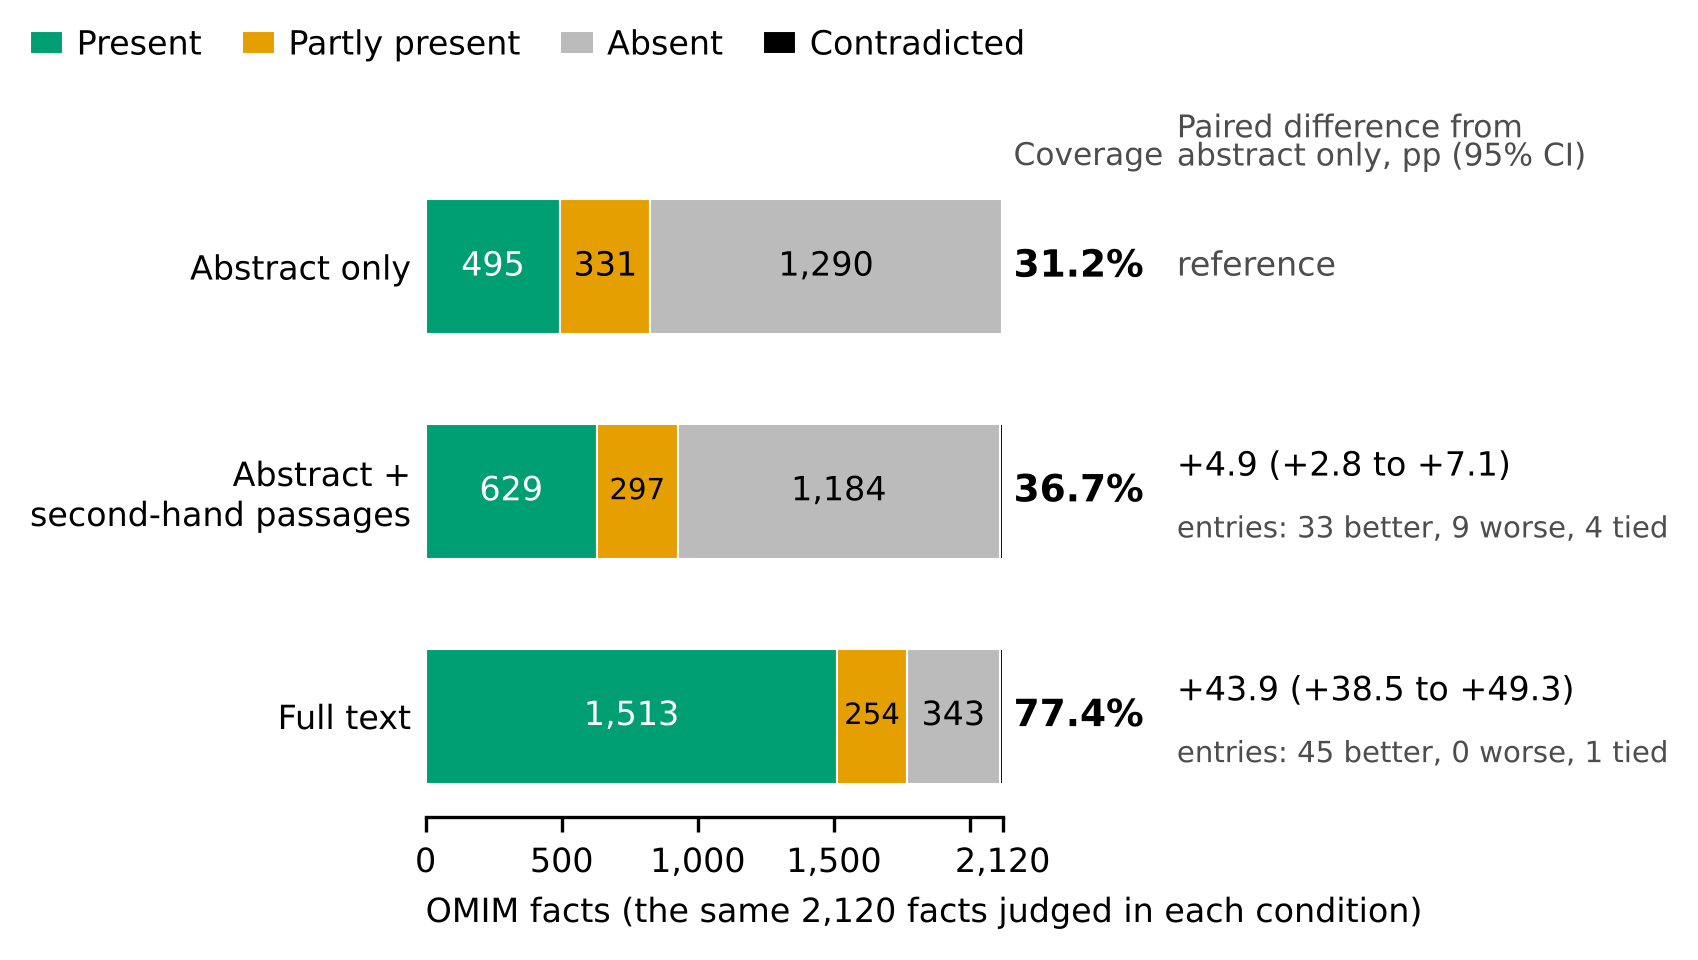
\includegraphics[width=\linewidth]{figures/fig_hidden_fulltext.png}
\caption{OMIM facts conveyed for the same papers with their full text hidden (46 entries, 136 curator paragraphs, the same 2,120 fixed facts in each condition). Coverage counts present facts plus half of partly present ones; contradicted facts (4, 10, 10) are too few to see. Right: paired difference in per-entry coverage from the abstract-only draft, bootstrap 95\% intervals. Only the full-text draft went through the repair round.}
\label{fig:hidden}
\end{minipage}\hfill
\begin{minipage}[t]{0.41\linewidth}
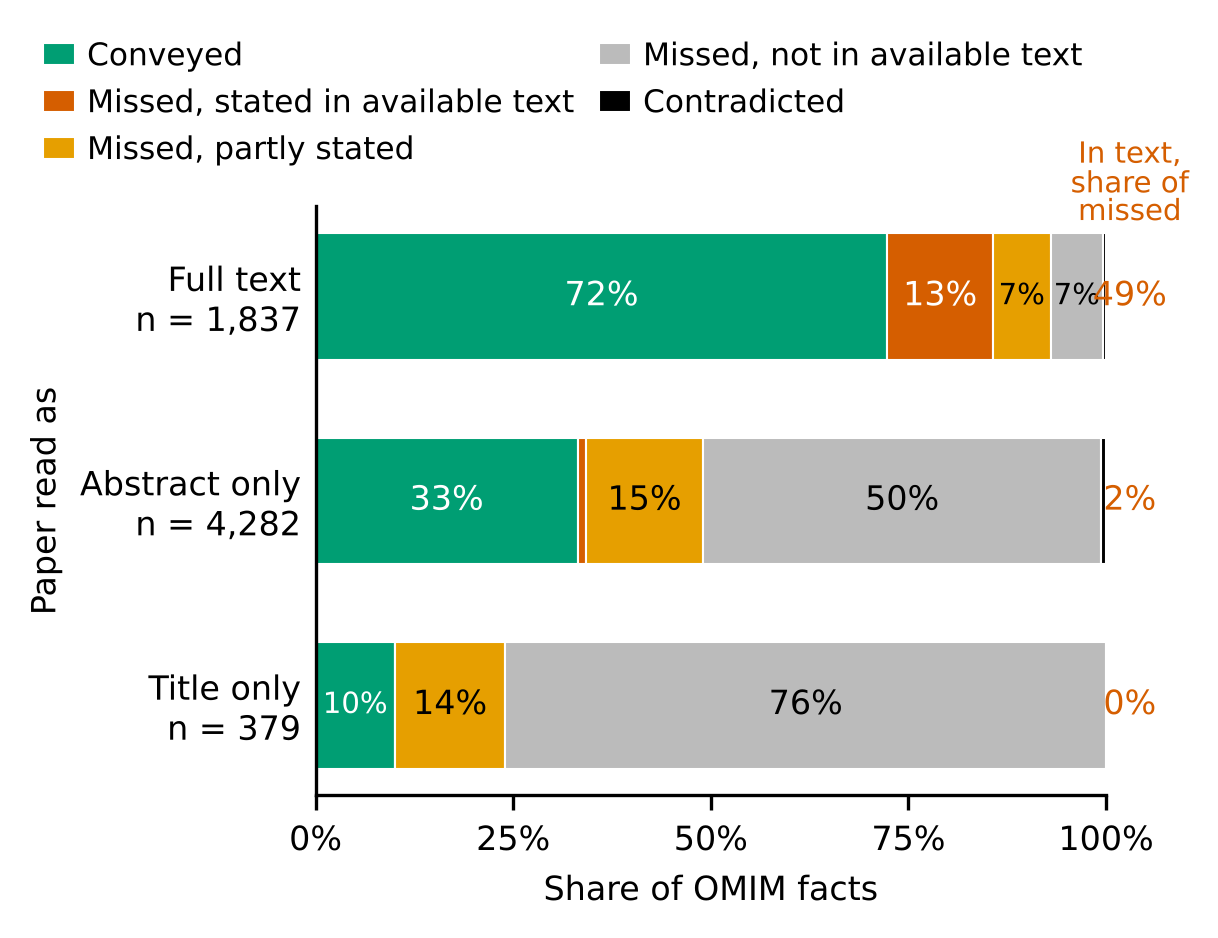
\includegraphics[width=\linewidth]{figures/fig_missed_facts.png}
\caption{Where the facts direct reading did not fully convey went, by access level (97 entries, 466 paragraphs). Each missed fact was checked once against the text available for its paper; the check is a model judgement. Partly conveyed facts count as missed; a small remainder were contradicted. Right: share of missed facts stated in the available text.}
\label{fig:missed}
\end{minipage}
\end{figure}

\textbf{Where the missed facts went.} Each fact that direct reading did not fully convey was checked against the text available for its paper (Figure~\ref{fig:missed}). For full-text papers, 245 of 501 missed facts (49\%) were stated in the text the model read; for abstract-only papers 46 of 2,837 (2\%), and for title-only papers none of 341. Over all 6,498 facts, 43\% were conveyed, 4\% were omitted although stated in the available text, 13\% were omitted and partly stated, and 40\% were not in the available text. Most of the shortfall is information the model was not given. The converse was not measured: direct reading conveys 40.1\% of the facts of abstract-only papers (pooled), and how many of those are stated in the abstract, rather than recalled from memory cued by it, is unknown; the memory-only control (Section~\ref{sec:memory}) does not bound such cued recall.

\subsection{Controlled comparison of the strategies}
\label{sec:main}
\textbf{Completion.} Of the 100 entries, 93 were completed by all six strategies; the memory-based strategies completed all 100, and the others lost one to three drafts or had incomplete entries (Appendix Table~\ref{tab:app_completion}).

\begin{table}[t]
\caption{Main comparison on the 93 entries every strategy completed. Facts: OMIM facts conveyed (primary endpoint, mean over entries). $\Delta$: paired difference from direct reading in points, bootstrap 95\% interval, and entries better/worse/tied. Remaining columns are secondary: claims judged supported (after repair, except for the memory-only control, which is audited but not repaired), synopsis HPO F1 (exact), OMIM variants recovered, variant precision, causal-gene F1 and inheritance match (\%). Subscripts give $n$ where fewer than 93 entries contribute.}
\label{tab:main}
\begin{center}
\footnotesize
\setlength{\tabcolsep}{2.2pt}
\begin{tabular}{lcccccccc}
\toprule
Strategy & Facts & $\Delta$ facts (95\% CI); b/w/t & Supp. & HPO F1 & Var.\ rec. & Var.\ prec. & Gene & Inher. \\
\midrule
\multicolumn{9}{l}{\emph{Read and write}} \\
Direct reading & 49.1 & --- & 96.1 & 35.9 & 66.5 & 88.7$_{82}$ & 97.5 & 93.5 \\
Agentic curator & 48.4 & $-0.6$ ($-1.3$, $+0.0$); 31/42/20 & 96.4 & 35.6 & 65.9 & 87.9$_{82}$ & 97.5 & 93.5 \\
\multicolumn{9}{l}{\emph{Extract, then write}} \\
Evidence graph & 48.6 & $-0.5$ ($-1.5$, $+0.5$); 33/45/15 & 96.5 & 34.6 & 65.9 & 76.9$_{87}$ & 98.2 & 92.5 \\
Case table first & 47.2 & $-1.9$ ($-3.1$, $-0.8$); 31/48/14 & 94.7 & 34.0 & 64.3 & 72.9$_{88}$ & 93.9 & 91.4 \\
\multicolumn{9}{l}{\emph{Memory first}} \\
Recall, then verify & 14.6 & $-34.5$ ($-39.2$, $-29.9$); 2/89/2 & 94.2$_{92}$ & 24.9 & 11.6 & 100.0$_{23}$ & 82.8 & 73.1 \\
\multicolumn{9}{l}{\emph{Control}} \\
Memory only & 15.1 & $-34.0$ ($-39.3$, $-28.7$); 7/85/1 & 50.8 & 30.6 & 15.2 & 97.2$_{30}$ & 83.9 & 82.8 \\
\bottomrule
\end{tabular}
\end{center}
\end{table}

\textbf{In this regime the reading strategies are close, and replicate noise is as large as their differences.} On the primary endpoint, direct reading, the evidence graph and the agentic curator lie within 0.7 points of one another (Table~\ref{tab:main}). To calibrate such differences, we repeated generation, audit and scoring three times on 30 entries (six per band): replicate noise alone gives a 95\% half-width of 1.0 point on a difference between two strategies over 93 entries (1.8 over 30), and judge variation is smaller (Appendix~\ref{app:stability}). A single run at this sample size therefore cannot rank the reading strategies. The evidence graph's $-0.5$ lies within this noise. The agentic curator's $-0.6$ has an interval that touches zero ($-1.3$ to $+0.0$), and its better/worse counts (31/42) lean negative. Only the case table's $-1.9$ ($-3.1$ to $-0.8$) exceeds the noise half-width. On the separate set of entries created June to November 2026 (20 compared), the ordering of the reading strategies is the same and all lie within 2.8 points of direct reading; there the agentic curator's interval excludes zero ($-1.1$, $-1.8$ to $-0.3$; Appendix~\ref{app:new}).

\textbf{Measurement choices move differences of this size.} An earlier analysis that excluded entries whose writer was stopped but scored entries with a stopped per-paper call placed the evidence graph 2.1 points below direct reading; under a symmetric completion rule the difference is not distinguishable from zero. Splitting the reference into facts afresh for each draft, the earlier scoring, gives levels 2--5 points higher than the fixed lists, with the same ordering (Appendix Table~\ref{tab:app_full}). Counting missing drafts as zero over all 100 entries gives intervals that are wide and include zero for all three reading strategies, for example $-3.0$ to $+3.1$ for the evidence graph (Appendix Table~\ref{tab:app_itt}).

\textbf{Secondary measures.} Extract-then-write raises synopsis recall at lower precision, with more terms per entry, and produces more variants that OMIM does not list (111 and 130 against 36), whether or not the paper reports them (Appendix Tables~\ref{tab:app_full} and~\ref{tab:app_varinh}). Recall, then verify keeps 94.2\% of claims judged supported but states no inheritance in 22 of 93 entries; since it may not add content from the papers, its low coverage is partly by construction. At list price for this one model, generation, audit and scoring cost \$1.15--\$1.18 for the read-and-write strategies and \$1.72--\$1.78 for extract-then-write per entry (Appendix Table~\ref{tab:app_cost}).


\begin{figure}[t]
\begin{minipage}[t]{0.49\linewidth}
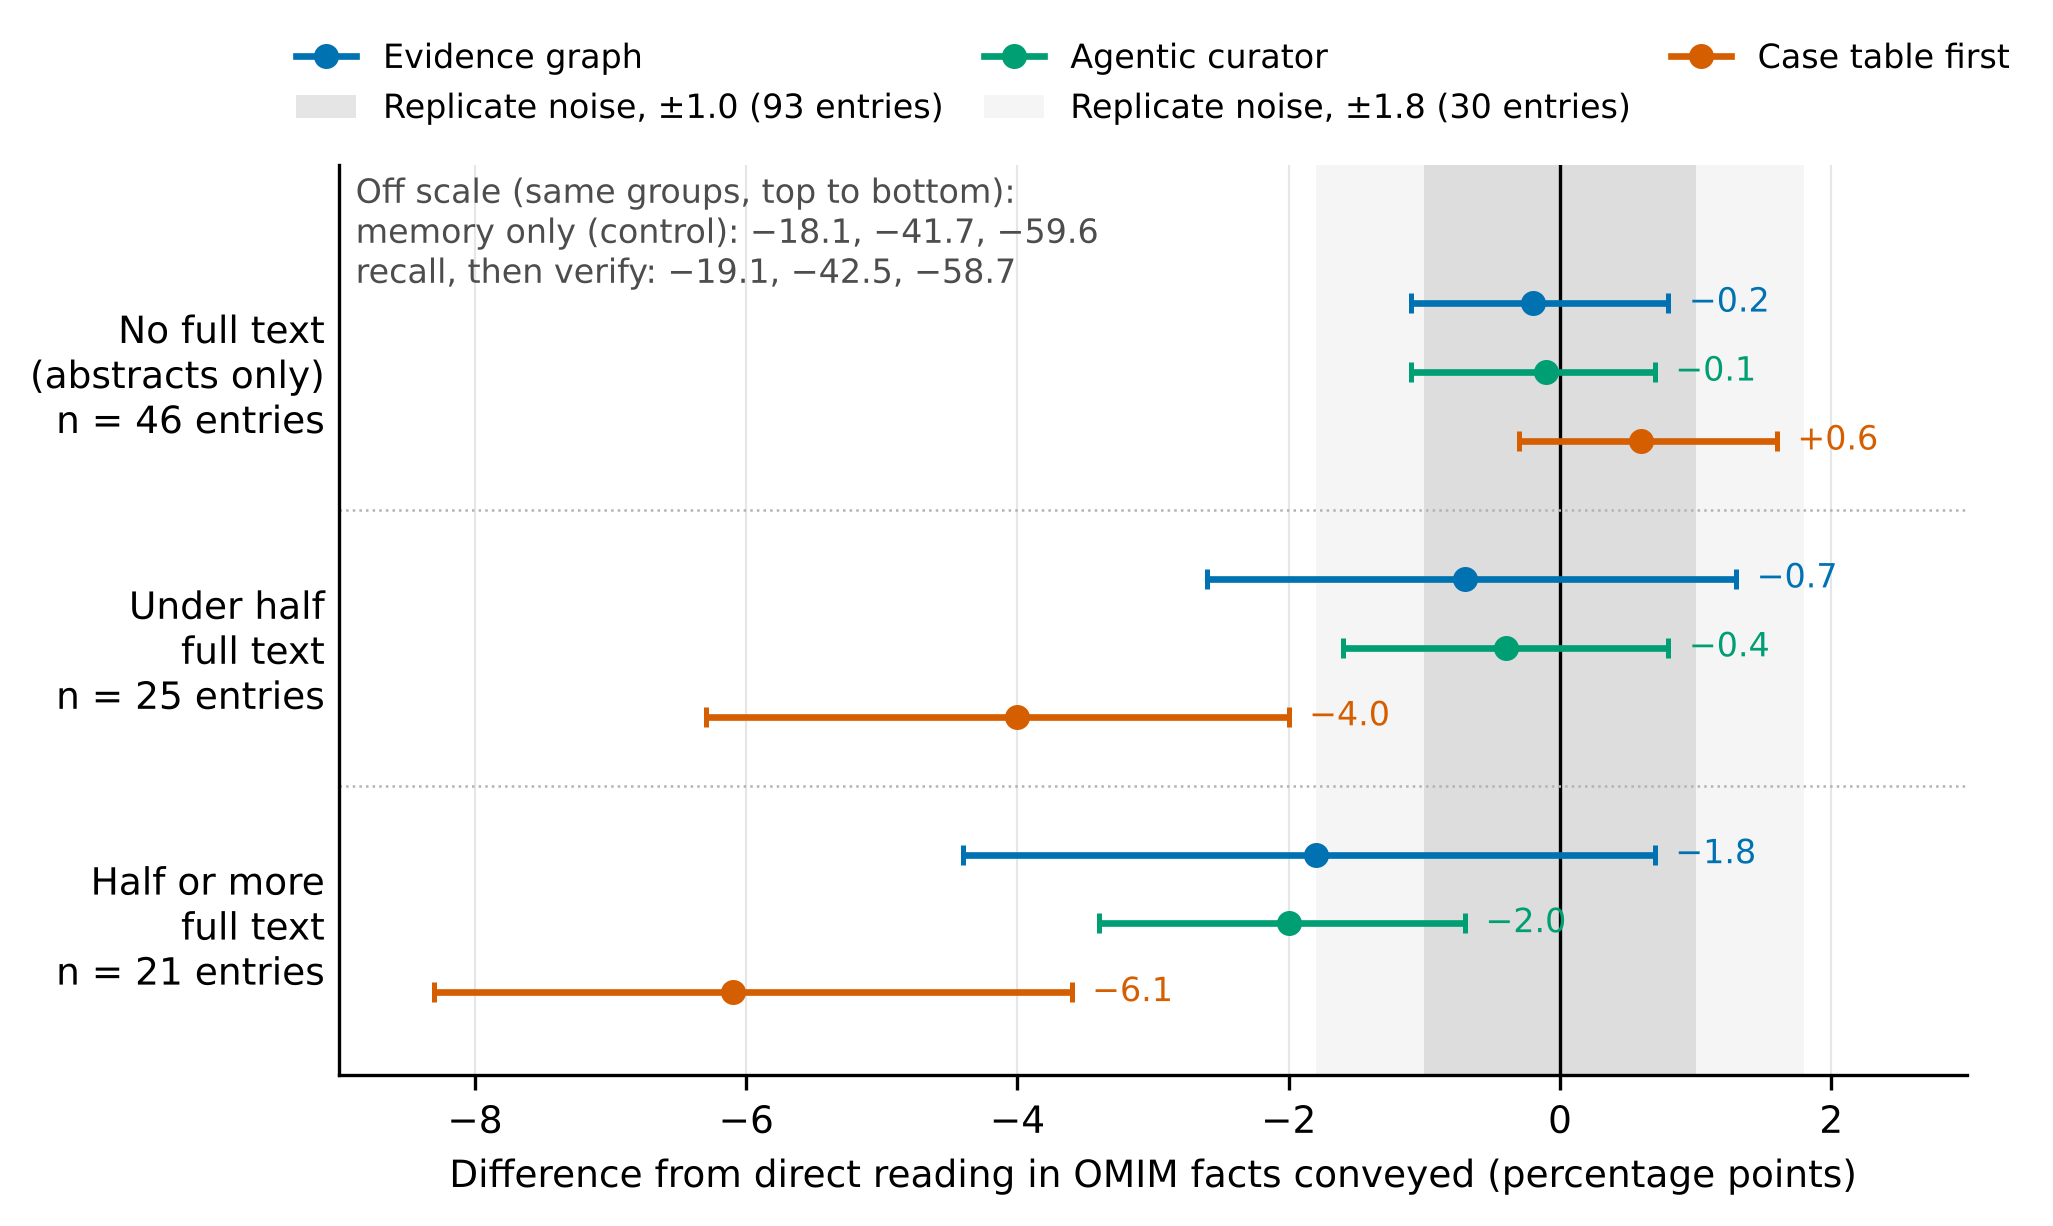
\includegraphics[width=\linewidth]{figures/fig_access_strata.png}
\caption{Paired difference from direct reading in OMIM facts conveyed (points; 95\% interval) by the share of an entry's references readable in full: none (46 entries), under half (25), half or more (21). Bands: replicate-noise half-width over 93 (1.0, dark) and 30 entries (1.8, light). Memory-based strategies are off scale. Observational and confounded with creation date and journal; the within-paper test is Figure~\ref{fig:hidden}.}
\label{fig:strata}
\end{minipage}\hfill
\begin{minipage}[t]{0.49\linewidth}
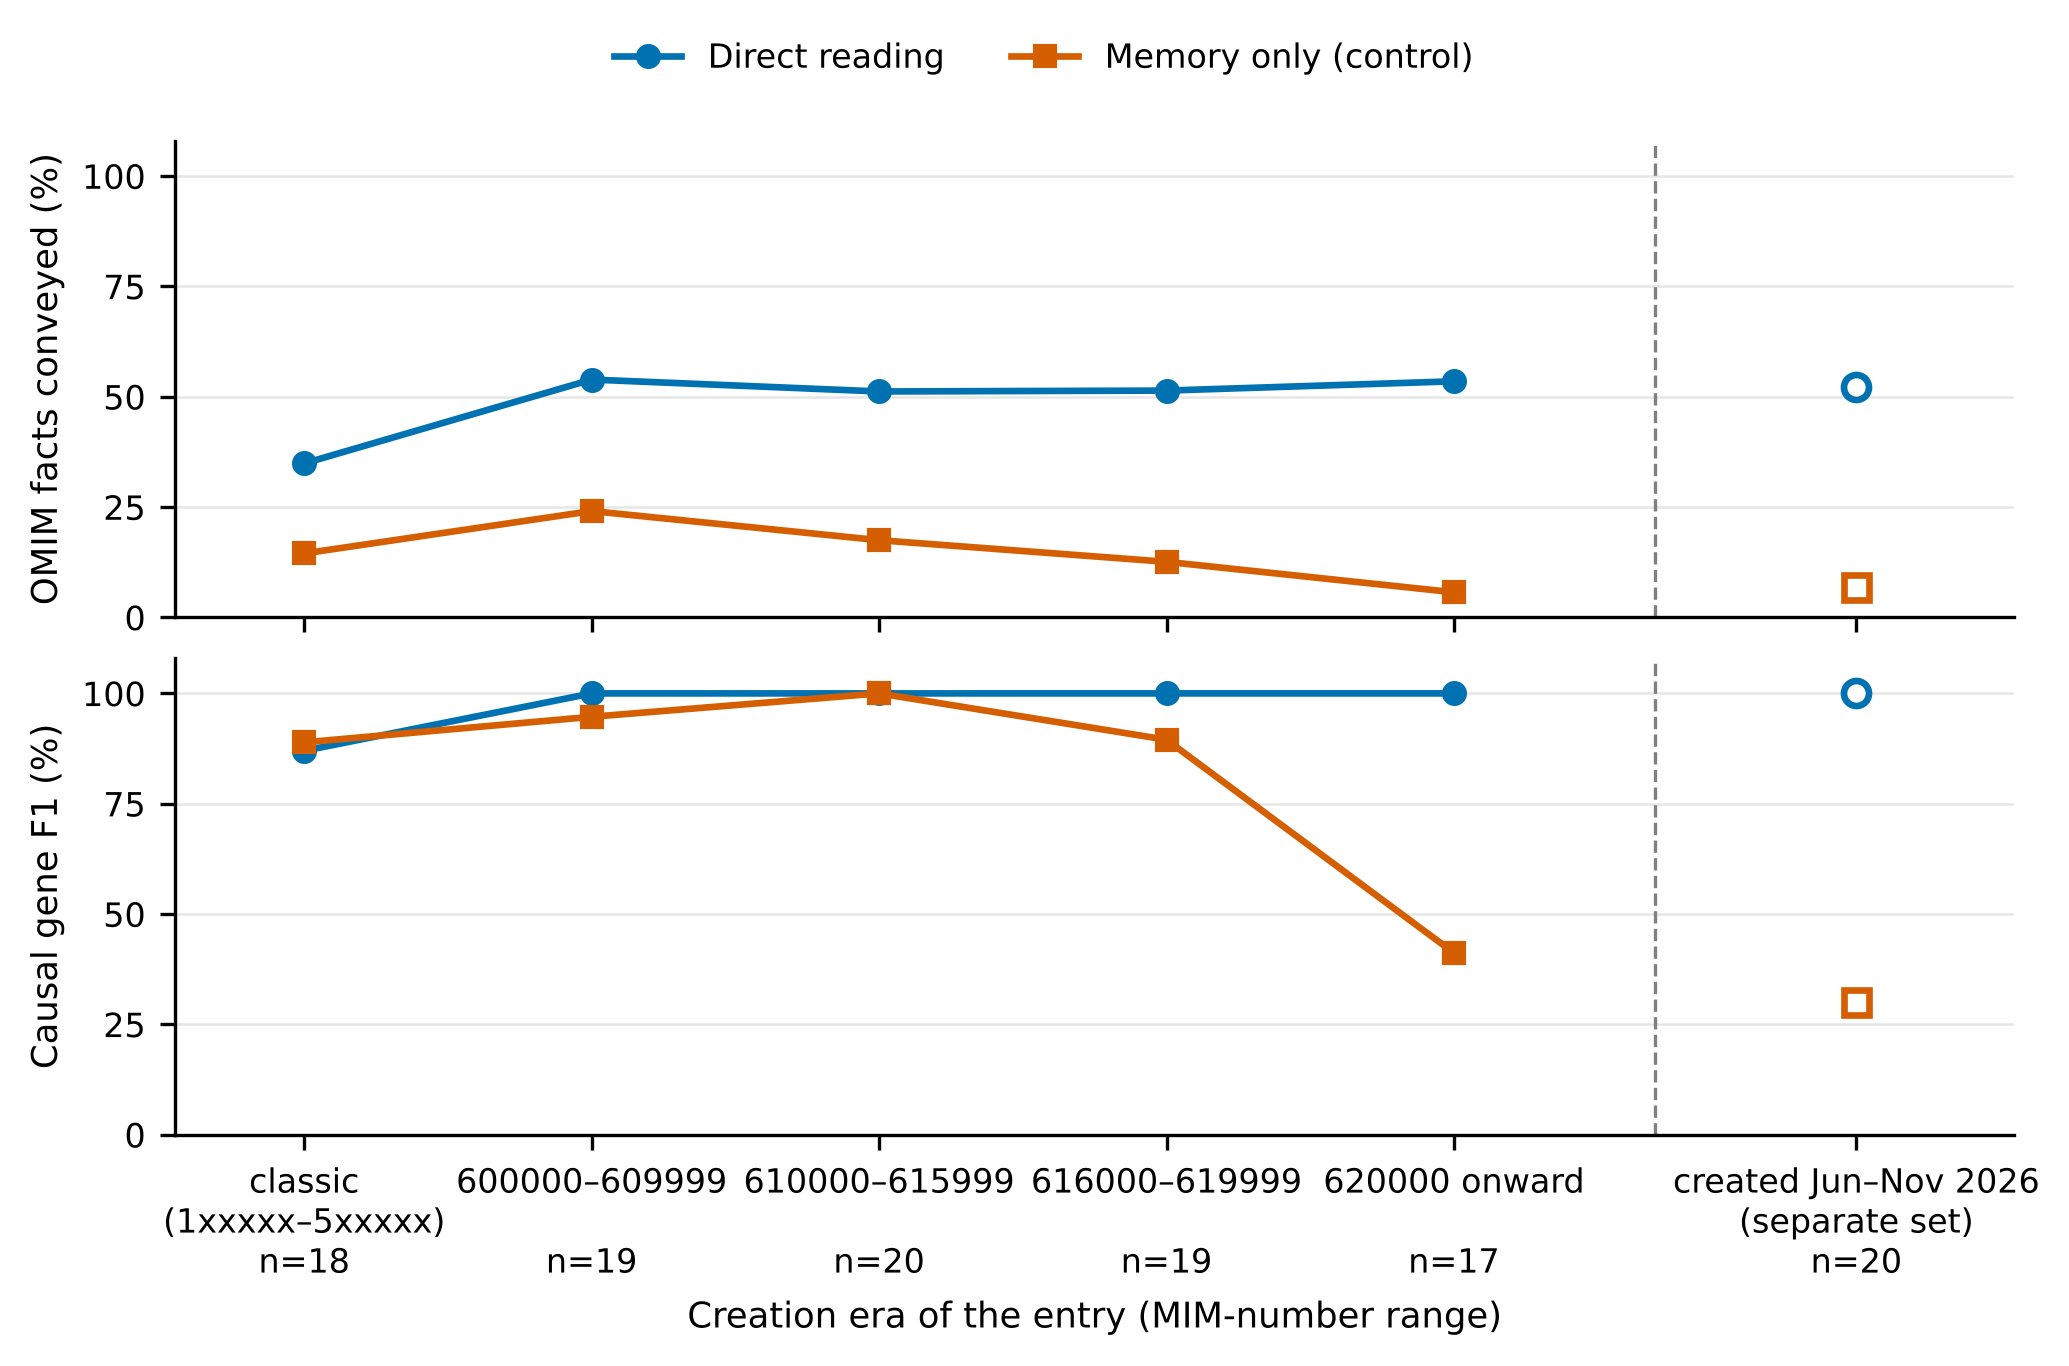
\includegraphics[width=\linewidth]{figures/fig_memory_by_era.png}
\caption{OMIM facts conveyed (top) and causal-gene F1 (bottom), memory-only control and direct reading, entry means by creation era ($n$ = 18, 19, 20, 19, 17). Hollow markers: 20 entries created June to November 2026. The model's training cut-off is not known; this is a contamination check, not proof that reading is free of memorisation.}
\label{fig:memory}
\end{minipage}
\end{figure}

\subsection{The strategies separate where more full text is readable}
\label{sec:strata}
Grouping entries by the share of their references readable in full (Figure~\ref{fig:strata}), the reading strategies are within noise of direct reading where no full text exists (46 entries) and separate as the share grows: where half or more is full text (21 entries), the case table trails by $-6.1$ points ($-8.3$ to $-3.6$) and the agentic curator by $-2.0$ ($-3.4$ to $-0.7$). Pooled over the facts of full-text papers, the case table trails direct reading by $-5.9$ points ($-9.0$ to $-2.9$; 40 entries; Appendix Table~\ref{tab:app_access}). This comparison is across different entries and papers, rests on few entries per group, and is confounded with entry creation date and journal.

\subsection{What the audit can and cannot see}
\label{sec:audit}
\textbf{What it removes.} The memory-only control has 50.8\% of claims judged supported and, before repair, 22.1\% unsupported but 0.6\% contradicted (pooled: 576 unsupported, 18 contradicted). Unsupported by the cited papers is not wrong: most flagged memory claims lack support rather than conflict with the papers. The read-and-write and extract-then-write strategies reach 94.7--96.5\%. In 60 paragraphs the audit had passed, one fact was altered by rule (a count, a zygosity, a residue or a mode of inheritance); the audit flagged all 60, each on a claim containing the altered value, and in 6 of the 60 also flagged other claims. This measures sensitivity to blunt single-fact substitutions only: no unaltered controls were run, so the false-flag rate was not measured, and omissions and misattributions were not tested.


\textbf{What it cannot see.} In the hidden-full-text experiment, the second-hand draft made 2,308 claims about the hidden papers, each audited against what the writer saw and against the paper's full text. Of the 112 claims whose supporting quote came from a later paper's passage, the full text supports 74, partly supports 24, does not support 11 and contradicts 3. Because our full texts exclude supplementary material, ``unsupported by the full text'' is an upper bound on error. An audit against the text the writer saw passes such second-hand support, and in general it checks fidelity to the cited text rather than correctness: a draft that faithfully copies a source's error passes. Re-examining by the same model the 37 facts on which a direct-reading draft contradicted the reference paragraph, the paper was judged to support the draft in 22, the reference in 1 and both in 1, with 13 undecidable from the readable text; these are unconfirmed leads, adjudicated by the model that had already passed the same claims.

\subsection{The memory-only control as a contamination check}
\label{sec:memory}
From the oldest to the newest band, the memory-only control conveys 14.5\%, 24.1\%, 17.5\%, 12.6\% and 5.7\% of facts, and its causal-gene F1 falls to 41.2\% for entries from 620000 onward (Figure~\ref{fig:memory}). On the 20 compared entries created June to November 2026, memory alone conveys 7.0\% of facts against 52.2\% for direct reading (paired difference $-45.2$, $-52.4$ to $-38.0$), and names the causal gene with an F1 of 30.0\% (Appendix~\ref{app:new}). Memory alone thus contributes little for the newest entries. The control does not show that the reading results are free of memorisation: within abstract-only papers, direct-reading coverage declines from 49.8\% for the 600000--609999 band to 37.9\% for entries from 620000 onward (33.0\% for the classic band).



\subsection{Matched ablation of the extract-then-write implementations}
\label{sec:ablation}
On 40 entries weighted towards full text (25 with at least half their papers readable in full), we varied our extract-then-write implementations. \emph{Matched} raises per-paper extraction to high effort and lets the writer choose synopsis terms (and, for the case table, inheritance) instead of fixed rules; the two changes were made together. \emph{Plus text} also gives the writer the papers' text. Thirty-eight entries were completed by all seven strategies; the safety filter stopped some high-effort extraction calls.

Matching moves the case table from $-2.3$ to $-0.2$ points against direct reading (matched minus original $+2.1$, $+1.1$ to $+3.2$) and the evidence graph from $+1.0$ ($-0.9$ to $+2.8$) to $+1.8$ ($+0.4$ to $+3.3$; Appendix Tables~\ref{tab:app_abl_means} and~\ref{tab:app_abl_diff}). Choosing synopsis terms cannot change which facts or variants are extracted, so we attribute the gain in facts to extraction effort; this attribution is an inference. Adding the papers' text raises claims judged supported ($+1.5$, $+0.9$ to $+2.1$, for the graph) but not facts ($+0.0$). The point estimates of synopsis precision stay below direct reading for every extract-then-write variant, at two to three times the generation cost. At least part of the case table's apparent deficit thus reflects extraction effort, a setting unrelated to its representation, rather than the table itself (Appendix~\ref{app:ablation}).

\subsection{Add-ons: one small gain with costs, and two nulls}
\label{sec:addons}
\textbf{Second-hand evidence} (96 entries; 361 of the 401 papers not readable in full received passages) raises OMIM facts conveyed by $+1.8$ points ($+1.0$ to $+2.8$; 49/31/16) and variants recovered by $+5.0$ ($+1.3$ to $+9.2$). It also raises unsupported claims before repair from 0.4\% to 3.9\% and facts contradicted ($+0.2$, $+0.0$ to $+0.5$), and lowers claims judged supported ($-1.8$, $-2.9$ to $-0.8$). \textbf{The learned curation guide} did not improve OMIM facts conveyed on its own training entries (final guide $+0.06$ points); on 68 of the 70 held-out entries it changed facts by $+1.0$ ($+0.0$ to $+2.0$; 30/25/13). With two reflection rounds on 27 entries, this null says nothing about better-resourced prompt optimisation. \textbf{Reconciliation} accepted 40 of 57 proposed merges of patient or family records in 27 entries and changed OMIM facts conveyed by $+0.1$ ($-0.1$ to $+0.4$; 97 entries) and no other score. A planted test merged 10 of 10 copied reports and no unrelated records, which shows only that a stated re-report is caught; the case database was not validated against external per-patient ground truth (Appendix~\ref{app:addons}).

\section{Discussion and Limitations}
\label{sec:discussion}
The closeness of the reading strategies holds in the regime tested: entries with 2--12 references, 19\% of papers readable in full, inputs that fit one prompt, and one model. It is not a claim that the method matters little in general: where more full text is readable the strategies separate, and larger inputs, other models and papers with supplements were not tested. The access effect is expected in direction; the benchmark adds its size within the same papers. The negative results for recall-then-verify (which, as implemented, cannot add content), the learned guide and reconciliation hold for the implementations and entry sizes tested.

\textbf{Measurement lessons.} Four observations bear on comparisons of document-to-text systems generally. Stopped replies must be handled symmetrically for one-call and per-paper strategies, or a spurious difference appears (2.1 points here). Fixed fact lists and per-draft splitting give different levels. Run-to-run noise of the whole pipeline is as large as the differences between reading strategies, so single-run comparisons at this sample size cannot rank them. And a matched ablation can show a pipeline's deficit depending on a setting other than its representation.

\textbf{Limitations.} (i) One model family wrote, audited and judged everything; no human has read any draft, verdict or fact judgement, so no judge is validated, and no second model family was tested, so whether the strategies stay close for other models is unknown. (ii) The reference is indirect and narrow: variant-centred curator paragraphs, an ontology annotation set from two sources, and gene and inheritance tables; narrative sections of entries are not compared, and a draft makes about twice as many statements about a paper as the paragraph has facts (24.0 against 11.9 for direct reading), so coverage is a lower bound on agreement with the entry, and draft content beyond the reference is checked only by the audit. (iii) Every strategy is given the curators' reference list; finding the literature was tested only on ten entries (Appendix~\ref{app:updates}). (iv) Only open-access text without supplementary material was available, where much variant and patient data in genetics papers lives; how much coverage of abstract-only papers comes from the abstract rather than from cued recall was not measured. (v) Variant names are not validated against reference sequences, and inheritance is compared as coarse classes. (vi) Strategies were developed on the same entries they are evaluated on; there is no separate development set, although the entries created June to November 2026 reproduce the ordering and closeness of the reading strategies. (vii) Stopped replies remove entries, unevenly across strategies. (viii) Entries with few references dominate and inputs too large for one prompt were not tested; the 30--75-reference tier has about ten comparable entries, mostly abstracts, and its fact score covers a minority of each entry's references, so it is exploratory (Appendix~\ref{app:large}). (ix) The audit's false-flag rate was not measured, and in the access experiment only the full-text arm was repaired. (x) Cost is at list price for one model.
%%%%%%%%% EXPERIMENTS %%%%%%%%%

\section{Conclusion}
\label{sec:conclusion}
%%%%%%%%% CONCLUSION %%%%%%%%%
We asked how much the generation strategy matters when everything else is fixed, what limits agreement with curators, and what a claim-level audit can see. On 100 OMIM entries with 2--12 references, written by one model from exactly the cited papers at current open access, the reading strategies are close, within or near a measured noise floor, and separate where more full text is readable. Access to the source bounds agreement: hiding the full text of the same papers lowers coverage of curator-written facts from 77.4\% to 31.2\%, many times any difference between reading strategies. The audit checks fidelity to the cited text, not correctness, and no judgement in the study was validated by a person. The benchmark, built only from public sources with fixed fact lists and per-entry release of drafts, verdicts and scores, makes these comparisons repeatable for other strategies and models.
%%%%%%%%% CONCLUSION %%%%%%%%%

\section*{Ethics Statement}
The benchmark is built from public resources (NCBI, ClinVar, HPO, MedGen, Europe PMC, HGNC). Curator-written text is used for scoring and is not redistributed; released score files carry fact identifiers and statuses, not wording, and rights holders' terms of use for curated text apply to anyone rebuilding the reference. No human subjects were involved, and no patient-level data beyond what published papers report were used. Generated entries are drafts for expert review and are not clinical guidance; they must be marked as machine generated and not as OMIM content. No curator has checked any draft, and the disagreements between drafts and the reference reported here are unconfirmed.

\section*{Reproducibility Statement}
Section~\ref{sec:method} specifies the entry sampling (fixed seed, five creation-era bands, eligibility rules), the reference sources, the strategies, guards, audit, scoring and statistics; Appendix~\ref{app:settings} lists the model settings and Appendix Table~\ref{tab:app_experiments} the entry sets of every experiment. One model (Claude Opus 5.5) was used through a command-line interface in headless mode with schema-constrained output; it exposes no temperature or seed, so exact regeneration is not guaranteed, and we instead report replicate and judge variation (Appendix~\ref{app:stability}). Replies are cached, so each call was made once. All experiments, pilots and re-scoring used 38,037 cached model calls, 253 million input and 69 million output tokens, about \$2,841 at list price. The curator-written text is not redistributed, but every part of the reference comes from public resources (ClinVar, HPO, MedGen), from which it can be rebuilt under the rights holders' terms of use; the released score files carry fact identifiers and statuses, not wording. The harness and per-entry drafts, verdicts and scores are released with the paper as supplementary material.

%%%%%%%%% REFERENCES %%%%%%%%%
\bibliography{references}
\bibliographystyle{iclr2025_conference}
%%%%%%%%% REFERENCES %%%%%%%%%

%%%%%%%%% Appendix %%%%%%%%%
\clearpage
\appendix
\FloatBarrier
\section{Experiments and entry sets}
\label{app:experiments}
\begin{table}[!htbp]
\caption{Every experiment, its entry set, the entries compared and why others dropped out. ``Stopped'': the writer's reply was stopped by the model's safety filter (no draft); ``per-paper call failed'': a per-paper call was lost (incomplete draft). Entries are compared only when every strategy in the comparison completed them.}
\label{tab:app_experiments}
\scriptsize
\begin{tabularx}{\linewidth}{>{\raggedright\arraybackslash}p{2.7cm}>{\raggedright\arraybackslash}p{3.3cm}>{\centering\arraybackslash}p{0.9cm}>{\raggedright\arraybackslash}X>{\raggedright\arraybackslash}p{1.1cm}}
\toprule
Experiment & Entry set & Compared & Why entries dropped out & Where \\
\midrule
Main comparison (six strategies) & 100 main entries (2--12 references, five creation-era bands) & 93 & 7 entries: no draft (direct reading 3, agentic curator 2, evidence graph 1); per-paper call failed (evidence graph 3, case table 3) & Sec.~\ref{sec:main}, App.~\ref{app:main} \\
Missing drafts as zero & 100 main entries & 100 & none; missing drafts scored zero & App.~\ref{app:main} \\
Strata by access & the 93 compared entries & 46 / 25 / 21 / 1 & grouped by share of references readable in full & Sec.~\ref{sec:strata} \\
Missed-fact attribution & 100 main entries, direct reading & 97 & 3 without a draft (writer stopped) & Sec.~\ref{sec:access} \\
Hidden full text & 49 main entries with papers readable in full (91 papers hidden) & 46 & 3 whose full-text direct-reading draft was stopped & Sec.~\ref{sec:access}, App.~\ref{app:hidden} \\
Judge variation & 30-entry replicate subset (six per band) & 30 & none & App.~\ref{app:stability} \\
Run-to-run replicates & 30-entry replicate subset, three replicates & 30 & none & App.~\ref{app:stability} \\
Matched ablation & 40 entries weighted to full text & 38 & high-effort extraction stopped (graph variants 1 each, table variants 2 each) & Sec.~\ref{sec:ablation}, App.~\ref{app:ablation} \\
Second-hand evidence & 100 main entries & 96 & not completed by both strategies & Sec.~\ref{sec:addons}, App.~\ref{app:hidden} \\
Reconciled case database & 100 main entries & 97 & not completed by both strategies & Sec.~\ref{sec:addons}, App.~\ref{app:addons} \\
Learned curation guide & 70 held-out main entries (guide learned on 27 of 30 training entries) & 68 & not completed by both strategies & Sec.~\ref{sec:addons}, App.~\ref{app:addons} \\
Entries created June--November 2026 & 30 newest of 53 eligible 2026 entries & 20 & stopped (agentic curator 6, direct reading 2); per-paper call failed (evidence graph 7, case table 10) & Sec.~\ref{sec:main}, App.~\ref{app:new} \\
30--75 references (exploratory) & 12 entries & 10 & 2 entries: no draft (direct reading 1, evidence graph 1); per-paper call failed (case table, both) & App.~\ref{app:large} \\
Planted errors & 60 paragraphs the audit had passed & 60 & none; no unaltered controls & Sec.~\ref{sec:audit} \\
Draft--reference disagreements & 37 facts a direct-reading draft contradicted & 37 & 13 undecidable from the readable text & Sec.~\ref{sec:audit} \\
Updates; retrieval without a reference list & 10 entries each (evidence graph only) & 10 & none & App.~\ref{app:updates} \\
\bottomrule
\end{tabularx}
\end{table}


\section{Strategies and settings}
\label{app:settings}
Table~\ref{tab:app_strategies} describes each strategy. Settings: one model for everything, Claude Opus 5.5 (\texttt{claude-opus-5-5}), called through the Claude Code command-line interface in headless mode with schema-constrained output; no temperature or seed is exposed. Reasoning effort is high for writers (direct reading, the graph and table writers, the agent, the memory draft) and medium for per-paper extraction in the evidence graph and the case table, for the audit and for all judging; the matched ablation raises per-paper extraction to high. The agentic strategy has read and search tools over a folder of the papers and nothing else. The agentic curator reports which papers it opened (self-reported; tool calls are not logged): in the 98 entries it wrote it reported opening every paper, and all 2,600 quotes it gave were found verbatim in the papers. The memory drafts that recall, then verify starts from are the memory-only control's drafts. Synopsis terms are assigned by a lexical search over the ontology's labels and synonyms that returns candidates, from which the model chooses; Lin similarity uses information content computed from the ontology's disease annotations, averaged in each direction to give precision and recall.

\begin{table}[!htbp]
\caption{The strategies: three paradigms, a control and three add-ons each tested against its parent.}
\label{tab:app_strategies}
\scriptsize
\begin{tabularx}{\linewidth}{>{\raggedright\arraybackslash}p{2.4cm}>{\centering\arraybackslash}X>{\centering\arraybackslash}X}
\toprule
Strategy & Paradigm & What it does \\
\midrule
Direct reading & Read and write & All papers in one prompt; the model writes the entry. Baseline. \\
Agentic curator & Read and write & The model works in a folder of the papers with read and search tools and must give a verbatim quote for every paragraph. \\
Evidence graph & Extract, then write & Quote-backed findings are extracted per paper (findings whose quote is not in the paper are discarded) and joined into a graph of papers, genes, variants, phenotypes and inheritance; the writer sees only the graph. Synopsis terms are computed from the graph by rule; inheritance is written by the writer. \\
Case table first & Extract, then write & One record per reported patient or family is extracted per paper and pooled; synopsis terms and inheritance are computed by rule, candidate genes are confirmed by the writer; the writer sees only the table. \\
Recall, then verify & Memory first & The model writes from memory; the draft is audited against the papers; a rewriter keeps supported claims, restates partly supported ones, corrects contradicted ones and deletes the rest. It may not add content from the papers. \\
Memory only & Control & The memory draft, with no papers. Audited, not repaired. \\
Second-hand evidence & Add-on to direct reading & For a paper not readable in full, passages from later open-access papers that cite and describe it are added, marked as second-hand, for the writer and the audit. \\
Reconciled case database & Add-on to the case table & A propose, verify, apply step merges the same patient, family or variant reported in several papers and settles conflicts. \\
Learned curation guide & Add-on to direct reading & A guide of general rules, learned in two reflection rounds from 27 training entries' omissions and extras, is appended to the writer's prompt; tested on 70 held-out entries. \\
\bottomrule
\end{tabularx}
\end{table}

\FloatBarrier
\section{Main comparison: full results}
\label{app:main}
\begin{table}[!htbp]
\caption{Completion on the 100 main entries. An entry is compared only when every strategy completed it in full; 93 qualify (left out: 118210, 300148, 609296, 617232, 620609, 621030, 621068).}
\label{tab:app_completion}
\scriptsize
\begin{tabularx}{\linewidth}{>{\raggedright\arraybackslash}p{2.6cm}>{\centering\arraybackslash}X>{\centering\arraybackslash}X>{\centering\arraybackslash}X}
\toprule
Strategy & Complete & Incomplete (a per-paper call failed) & No draft \\
\midrule
Evidence graph & 96 & 3: 118210 (1 paper), 617232 (1 paper), 621030 (1 paper) & 1: 620609 \\
Direct reading & 97 & 0 & 3: 609296, 620609, 621068 \\
Agentic curator & 98 & 0 & 2: 609296, 620609 \\
Memory only (control) & 100 & 0 & 0 \\
Recall, then verify & 100 & 0 & 0 \\
Case table first & 97 & 3: 300148 (1 paper), 617232 (2 papers), 621068 (1 paper) & 0 \\
\bottomrule
\end{tabularx}
\end{table}

\begin{table}[!htbp]
\caption{All measures, means over the 93 compared entries ($\uparrow$ higher is better, $\downarrow$ lower is better). The primary endpoint is OMIM facts conveyed; the others are secondary. The row ``facts split afresh for each draft'' is the earlier scoring, which runs 2--5 points higher and gives the same ordering.}
\label{tab:app_full}
\scriptsize
\begin{tabularx}{\linewidth}{>{\raggedright\arraybackslash}p{4.2cm}>{\centering\arraybackslash}X>{\centering\arraybackslash}X>{\centering\arraybackslash}X>{\centering\arraybackslash}X>{\centering\arraybackslash}X>{\centering\arraybackslash}X}
\toprule
Metric & Evidence graph & Direct reading & Agentic curator & Memory only (control) & Recall, then verify & Case table first \\
\midrule
Claims supported by cited paper $\uparrow$ & 96.5\% & 96.1\% & 96.4\% & 50.8\% & 94.2\% (n=92) & 94.7\% \\
\ldots{} unsupported, before the repair round $\downarrow$ & 0.2\% & 0.2\% & 0.1\% & 22.1\% & 0.6\% (n=92) & 0.3\% \\
\ldots{} contradicted, before the repair round $\downarrow$ & 0.1\% & 0.0\% & 0.0\% & 0.6\% & 0.1\% (n=92) & 0.0\% \\
OMIM per-paper facts conveyed (primary endpoint) $\uparrow$ & 48.6\% & 49.1\% & 48.4\% & 15.1\% & 14.6\% & 47.2\% \\
\ldots{} fully (no partial credit) $\uparrow$ & 42.0\% & 42.4\% & 41.9\% & 10.2\% & 10.1\% & 40.8\% \\
OMIM per-paper facts contradicted $\downarrow$ & 0.4\% & 0.4\% & 0.4\% & 0.5\% & 0.3\% & 0.5\% \\
\ldots{} facts split afresh for each draft (earlier scoring) $\uparrow$ & 51.5\% & 52.1\% & 51.3\% & 20.4\% & 18.2\% & 49.3\% \\
Clinical synopsis HPO F1, exact $\uparrow$ & 34.6\% & 35.9\% & 35.6\% & 30.6\% & 24.9\% & 34.0\% \\
\ldots{} precision $\uparrow$ & 40.6\% & 44.1\% & 45.5\% & 53.5\% (n=92) & 53.6\% (n=87) & 40.7\% \\
\ldots{} recall $\uparrow$ & 37.4\% & 36.2\% & 34.2\% & 24.1\% & 18.4\% & 37.7\% \\
Clinical synopsis HPO F1, hierarchical $\uparrow$ & 54.7\% & 56.1\% & 56.2\% & 48.2\% & 40.5\% & 53.7\% \\
OMIM allelic variants recovered $\uparrow$ & 65.9\% & 66.5\% & 65.9\% & 15.2\% & 11.6\% & 64.3\% \\
Generated variants that are OMIM variants (precision) $\uparrow$ & 76.9\% (n=87) & 88.7\% (n=82) & 87.9\% (n=82) & 97.2\% (n=30) & 100.0\% (n=23) & 72.9\% (n=88) \\
Causal gene F1 $\uparrow$ & 98.2\% & 97.5\% & 97.5\% & 83.9\% & 82.8\% & 93.9\% \\
\ldots{} recall $\uparrow$ & 98.4\% & 97.3\% & 97.3\% & 83.9\% & 82.8\% & 94.1\% \\
Inheritance matches OMIM $\uparrow$ & 92.5\% & 93.5\% & 93.5\% & 82.8\% & 73.1\% & 91.4\% \\
OMIM references used $\uparrow$ & 94.6\% & 94.4\% & 93.3\% & 33.6\% & 65.2\% & 94.6\% \\
\bottomrule
\end{tabularx}
\vspace{4pt}
\begin{tabularx}{\linewidth}{>{\raggedright\arraybackslash}p{4.2cm}>{\centering\arraybackslash}X>{\centering\arraybackslash}X>{\centering\arraybackslash}X>{\centering\arraybackslash}X>{\centering\arraybackslash}X>{\centering\arraybackslash}X}
\toprule
Metric & Evidence graph & Direct reading & Agentic curator & Memory only (control) & Recall, then verify & Case table first \\
\midrule
Claims audited per entry & 113.5 & 101.0 & 97.3 & 28.2 & 26.3 & 117.9 \\
Claims that could not be audited per entry & 1.2 & 0.6 & 0.3 & 0.0 & 0.0 & 0.4 \\
Clinical-synopsis HPO terms per entry & 19.2 & 15.4 & 13.8 & 6.2 & 4.4 & 21.0 \\
Allelic variants per entry & 3.9 & 3.2 & 3.2 & 0.4 & 0.3 & 4.1 \\
\bottomrule
\end{tabularx}
\end{table}

\begin{table}[!htbp]
\caption{Paired differences from direct reading on the 93 compared entries: points, bootstrap 95\% interval, entries better/worse/same.}
\label{tab:app_paired}
\scriptsize
\begin{tabularx}{\linewidth}{>{\raggedright\arraybackslash}p{3.0cm}>{\centering\arraybackslash}X>{\centering\arraybackslash}X>{\centering\arraybackslash}X>{\centering\arraybackslash}X>{\centering\arraybackslash}X}
\toprule
Metric & Evidence graph & Agentic curator & Memory only (control) & Recall, then verify & Case table first \\
\midrule
Claims supported by cited paper $\uparrow$ & +0.4 ($-$0.4 to +1.3); 41/45/7 & +0.3 ($-$0.4 to +1.0); 53/33/7 & $-$45.3 ($-$50.3 to $-$40.3); 2/90/1 & $-$1.9 ($-$3.5 to $-$0.4); 34/53/5 (n=92) & $-$1.4 ($-$2.7 to $-$0.4); 34/56/3 \\
\ldots{} same, before the repair round $\downarrow$ & +0.0 ($-$0.3 to +0.2); 10/12/71 & $-$0.1 ($-$0.4 to +0.1); 11/8/74 & +22.4 (+18.3 to +26.7); 1/79/13 & +0.4 ($-$0.0 to +0.9); 10/10/72 (n=92) & +0.1 ($-$0.2 to +0.4); 12/18/63 \\
OMIM per-paper facts conveyed (primary) $\uparrow$ & $-$0.5 ($-$1.5 to +0.5); 33/45/15 & $-$0.6 ($-$1.3 to +0.0); 31/42/20 & $-$34.0 ($-$39.3 to $-$28.7); 7/85/1 & $-$34.5 ($-$39.2 to $-$29.9); 2/89/2 & $-$1.9 ($-$3.1 to $-$0.8); 31/48/14 \\
OMIM per-paper facts contradicted $\downarrow$ & +0.0 ($-$0.1 to +0.2); 8/5/80 & +0.0 ($-$0.1 to +0.2); 3/5/85 & +0.1 ($-$0.2 to +0.5); 17/14/62 & $-$0.1 ($-$0.2 to +0.2); 16/7/70 & +0.1 ($-$0.1 to +0.3); 5/8/80 \\
Clinical synopsis HPO F1, exact $\uparrow$ & $-$1.3 ($-$3.3 to +0.6); 34/45/14 & $-$0.3 ($-$1.5 to +0.8); 38/32/23 & $-$5.3 ($-$9.2 to $-$1.5); 41/52/0 & $-$11.0 ($-$14.4 to $-$7.6); 25/63/5 & $-$2.0 ($-$3.9 to $-$0.1); 39/45/9 \\
Clinical synopsis HPO F1, hierarchical $\uparrow$ & $-$1.4 ($-$2.8 to $-$0.1); 36/44/13 & +0.0 ($-$1.0 to +1.1); 40/35/18 & $-$7.9 ($-$12.3 to $-$3.5); 38/54/1 & $-$15.7 ($-$19.9 to $-$11.5); 21/68/4 & $-$2.5 ($-$4.1 to $-$0.9); 34/51/8 \\
OMIM allelic variants recovered $\uparrow$ & $-$0.5 ($-$3.1 to +2.5); 4/8/81 & $-$0.6 ($-$2.2 to +0.7); 3/3/87 & $-$51.3 ($-$60.0 to $-$42.4); 3/69/21 & $-$54.9 ($-$62.8 to $-$47.0); 0/71/22 & $-$2.2 ($-$4.9 to +0.3); 6/11/76 \\
Causal gene F1 $\uparrow$ & +0.7 (+0.0 to +2.1); 1/0/92 & +0.0 (+0.0 to +0.0); 0/0/93 & $-$13.6 ($-$21.5 to $-$6.1); 2/15/76 & $-$14.7 ($-$22.6 to $-$7.5); 1/15/77 & $-$3.6 ($-$8.6 to +0.4); 1/4/88 \\
Inheritance matches OMIM $\uparrow$ & $-$1.1 ($-$5.4 to +2.1); 1/2/90 & +0.0 ($-$3.2 to +3.2); 1/1/91 & $-$10.8 ($-$19.4 to $-$2.1); 3/13/77 & $-$20.4 ($-$29.0 to $-$11.8); 1/20/72 & $-$2.1 ($-$8.6 to +4.3); 4/6/83 \\
\bottomrule
\end{tabularx}
\end{table}

\begin{table}[!htbp]
\caption{Sensitivity analysis (intention to treat): all 100 entries, a missing draft counted as zero on each higher-is-better measure with a reference; incomplete drafts kept as scored; lower-is-better measures averaged over existing drafts. Missing drafts: evidence graph 1, direct reading 3, agentic curator 2. Bottom: paired differences from direct reading with interval, median, better/worse/tie and exact sign-test $p$.}
\label{tab:app_itt}
\scriptsize
\begin{tabularx}{\linewidth}{>{\raggedright\arraybackslash}p{3.4cm}>{\centering\arraybackslash}X>{\centering\arraybackslash}X>{\centering\arraybackslash}X>{\centering\arraybackslash}X>{\centering\arraybackslash}X>{\centering\arraybackslash}X}
\toprule
Metric & Evidence graph & Direct reading & Agentic curator & Memory only (control) & Recall, then verify & Case table first \\
\midrule
Claims supported by cited paper $\uparrow$ & 95.7\% & 93.2\% & 94.5\% (n=99) & 51.5\% & 94.4\% (n=98) & 94.5\% (n=99) \\
\ldots{} same, before the repair round $\downarrow$ & 0.3\% (n=99) & 0.4\% (n=97) & 0.2\% (n=97) & 22.8\% & 0.7\% (n=98) & 0.7\% (n=99) \\
OMIM per-paper facts conveyed (primary endpoint) $\uparrow$ & 48.4\% & 48.5\% & 48.9\% & 14.8\% & 14.2\% & 47.1\% \\
OMIM per-paper facts contradicted $\downarrow$ & 0.5\% (n=99) & 0.4\% (n=97) & 0.4\% (n=98) & 0.5\% & 0.3\% & 0.5\% \\
Clinical synopsis HPO F1, exact $\uparrow$ & 33.8\% & 34.6\% & 34.8\% & 29.4\% & 23.9\% & 33.3\% \\
Clinical synopsis HPO F1, hierarchical $\uparrow$ & 54.1\% & 54.6\% & 55.3\% & 46.7\% & 39.4\% & 52.9\% \\
OMIM allelic variants recovered $\uparrow$ & 65.8\% & 65.6\% & 66.1\% & 15.1\% & 11.3\% & 63.9\% \\
Causal gene F1 $\uparrow$ & 97.3\% & 94.7\% & 95.7\% & 83.0\% & 82.0\% & 92.3\% \\
Inheritance matches OMIM $\uparrow$ & 91.0\% & 91.0\% & 91.0\% & 82.0\% & 73.0\% & 90.0\% \\
\bottomrule
\end{tabularx}
\vspace{4pt}
\tiny
\begin{tabularx}{\linewidth}{>{\raggedright\arraybackslash}p{2.2cm}>{\centering\arraybackslash}X>{\centering\arraybackslash}X>{\centering\arraybackslash}X>{\centering\arraybackslash}X>{\centering\arraybackslash}X}
\toprule
Metric & Evidence graph & Agentic curator & Memory only (control) & Recall, then verify & Case table first \\
\midrule
Claims supported by cited paper $\uparrow$ & +2.4 (+0.1 to +5.6); median +0.0; 46/46/8; p 1.000 & +0.3 ($-$0.4 to +1.0); median +0.7; 56/34/9; p 0.026 (n=99) & $-$41.8 ($-$47.5 to $-$35.8); median $-$44.5; 4/94/2; p <0.001 & +0.2 ($-$2.5 to +3.7); median $-$1.2; 38/55/5; p 0.097 (n=98) & +0.3 ($-$2.2 to +3.6); median $-$1.0; 36/60/3; p 0.018 (n=99) \\
\ldots{} same, before the repair round $\downarrow$ & $-$0.1 ($-$0.4 to +0.2); median +0.0; 11/12/74; p 1.000 (n=97) & $-$0.2 ($-$0.5 to +0.1); median +0.0; 12/9/76; p 0.664 (n=97) & +21.9 (+18.0 to +26.1); median +17.2; 1/82/14; p <0.001 (n=97) & +0.3 ($-$0.2 to +0.8); median +0.0; 11/10/75; p 1.000 (n=96) & +0.4 ($-$0.3 to +1.3); median +0.0; 13/19/65; p 0.377 (n=97) \\
OMIM per-paper facts conveyed (primary) $\uparrow$ & $-$0.2 ($-$3.0 to +3.1); median +0.0; 36/48/16; p 0.230 & +0.4 ($-$1.0 to +2.7); median +0.0; 34/43/23; p 0.362 & $-$33.7 ($-$38.9 to $-$28.5); median $-$34.4; 9/89/2; p <0.001 & $-$34.3 ($-$39.2 to $-$29.6); median $-$32.9; 4/93/3; p <0.001 & $-$1.4 ($-$4.2 to +1.4); median $-$0.7; 34/51/15; p 0.082 \\
OMIM per-paper facts contradicted $\downarrow$ & +0.0 ($-$0.1 to +0.2); median +0.0; 9/6/82; p 0.607 (n=97) & +0.0 ($-$0.1 to +0.1); median +0.0; 4/5/88; p 1.000 (n=97) & +0.1 ($-$0.3 to +0.4); median +0.0; 19/14/64; p 0.487 (n=97) & $-$0.1 ($-$0.3 to +0.1); median +0.0; 18/8/71; p 0.075 (n=97) & +0.1 ($-$0.1 to +0.3); median +0.0; 7/8/82; p 1.000 (n=97) \\
Clinical synopsis HPO F1, exact $\uparrow$ & $-$0.8 ($-$2.8 to +1.3); median +0.0; 36/48/16; p 0.230 & +0.2 ($-$1.2 to +1.8); median +0.0; 40/35/25; p 0.644 & $-$5.2 ($-$8.9 to $-$1.5); median $-$2.7; 44/55/1; p 0.315 & $-$10.6 ($-$14.1 to $-$7.3); median $-$8.6; 27/67/6; p <0.001 & $-$1.3 ($-$3.5 to +0.9); median +0.0; 42/48/10; p 0.598 \\
Clinical synopsis HPO F1, hierarchical $\uparrow$ & $-$0.5 ($-$2.4 to +1.8); median +0.0; 38/48/14; p 0.332 & +0.7 ($-$0.8 to +2.5); median +0.0; 44/36/20; p 0.434 & $-$7.9 ($-$12.3 to $-$3.6); median $-$5.0; 40/58/2; p 0.085 & $-$15.3 ($-$19.5 to $-$11.1); median $-$11.6; 23/72/5; p <0.001 & $-$1.7 ($-$4.1 to +1.0); median $-$0.7; 36/55/9; p 0.059 \\
OMIM allelic variants recovered $\uparrow$ & +0.2 ($-$4.0 to +4.9); median +0.0; 7/10/83; p 0.629 & +0.5 ($-$1.6 to +3.1); median +0.0; 4/3/93; p 1.000 & $-$50.5 ($-$58.7 to $-$41.9); median $-$50.0; 3/73/24; p <0.001 & $-$54.3 ($-$62.1 to $-$46.4); median $-$60.0; 0/75/25; p <0.001 & $-$1.7 ($-$6.0 to +2.7); median +0.0; 8/14/78; p 0.286 \\
Causal gene F1 $\uparrow$ & +2.7 (+0.0 to +6.0); median +0.0; 3/0/97; p 0.250 & +1.0 (+0.0 to +3.0); median +0.0; 1/0/99; p 1.000 & $-$11.7 ($-$19.7 to $-$4.0); median +0.0; 3/15/82; p 0.007 & $-$12.7 ($-$20.0 to $-$5.7); median +0.0; 2/15/83; p 0.002 & $-$2.3 ($-$8.0 to +3.0); median +0.0; 3/5/92; p 0.727 \\
Inheritance matches OMIM $\uparrow$ & +0.0 ($-$4.0 to +4.0); median +0.0; 2/2/96; p 1.000 & +0.0 ($-$3.0 to +3.0); median +0.0; 1/1/98; p 1.000 & $-$9.0 ($-$17.0 to $-$1.0); median +0.0; 4/13/83; p 0.049 & $-$18.0 ($-$27.0 to $-$10.0); median +0.0; 2/20/78; p <0.001 & $-$1.0 ($-$8.0 to +6.0); median +0.0; 6/7/87; p 1.000 \\
\bottomrule
\end{tabularx}
\end{table}

\begin{table}[!htbp]
\caption{Pooled counts of audited claims and OMIM facts on the 93 compared entries.}
\label{tab:app_pooled}
\scriptsize
\begin{tabularx}{\linewidth}{>{\raggedright\arraybackslash}p{3.4cm}>{\centering\arraybackslash}X>{\centering\arraybackslash}X>{\centering\arraybackslash}X>{\centering\arraybackslash}X>{\centering\arraybackslash}X>{\centering\arraybackslash}X}
\toprule
 & Evidence graph & Direct reading & Agentic curator & Memory only (control) & Recall, then verify & Case table first \\
\midrule
Claims audited & 10,552 & 9,390 & 9,051 & 2,624 & 2,448 & 10,969 \\
\ldots{} supported & 10,227 & 9,069 & 8,802 & 1,343 & 2,308 & 10,497 \\
\ldots{} partly supported & 325 & 321 & 248 & 687 & 140 & 472 \\
\ldots{} unsupported & 0 & 0 & 1 & 576 & 0 & 0 \\
\ldots{} contradicted & 0 & 0 & 0 & 18 & 0 & 0 \\
Claims audited before repair & 10,526 & 9,371 & 9,056 & 2,624 & 2,448 & 10,945 \\
\ldots{} unsupported before repair & 20 & 17 & 10 & 576 & 13 & 21 \\
\ldots{} contradicted before repair & 8 & 0 & 2 & 18 & 4 & 4 \\
OMIM facts scored & 6,239 & 6,239 & 6,239 & 6,239 & 6,239 & 6,239 \\
\ldots{} conveyed & 2,562 & 2,620 & 2,593 & 502 & 502 & 2,490 \\
\ldots{} partly conveyed & 811 & 820 & 796 & 578 & 553 & 769 \\
\ldots{} missing & 2,840 & 2,771 & 2,820 & 5,133 & 5,167 & 2,948 \\
\ldots{} contradicted & 26 & 28 & 30 & 26 & 17 & 32 \\
\bottomrule
\end{tabularx}
\end{table}

\begin{table}[!htbp]
\caption{Allelic-variant precision (pooled) and inheritance errors by kind on the 93 compared entries. Precision counts a variant OMIM does not list as a miss whether or not the paper reports it.}
\label{tab:app_varinh}
\scriptsize
\begin{tabularx}{\linewidth}{>{\raggedright\arraybackslash}p{3.8cm}>{\centering\arraybackslash}X>{\centering\arraybackslash}X>{\centering\arraybackslash}X>{\centering\arraybackslash}X>{\centering\arraybackslash}X>{\centering\arraybackslash}X}
\toprule
 & Evidence graph & Direct reading & Agentic curator & Memory only (control) & Recall, then verify & Case table first \\
\midrule
Variants generated & 365 & 295 & 300 & 40 & 28 & 381 \\
\ldots{} matching an OMIM variant of the entry & 253 & 258 & 259 & 38 & 28 & 250 \\
\ldots{} listed by OMIM only from a paper outside the entry's references & 1 & 1 & 1 & 1 & 0 & 1 \\
\ldots{} not in OMIM & 111 & 36 & 40 & 1 & 0 & 130 \\
Pooled precision (entries where OMIM lists variants) & 69.3\% & 87.5\% & 86.3\% & 95.0\% & 100.0\% & 65.6\% \\
\bottomrule
\end{tabularx}
\vspace{4pt}
\begin{tabularx}{\linewidth}{>{\raggedright\arraybackslash}p{3.8cm}>{\centering\arraybackslash}X>{\centering\arraybackslash}X>{\centering\arraybackslash}X>{\centering\arraybackslash}X>{\centering\arraybackslash}X>{\centering\arraybackslash}X}
\toprule
 & Evidence graph & Direct reading & Agentic curator & Memory only (control) & Recall, then verify & Case table first \\
\midrule
Entries with an OMIM mode of inheritance & 93 & 93 & 93 & 93 & 93 & 93 \\
\ldots{} matched & 86 & 87 & 87 & 77 & 68 & 85 \\
\ldots{} none stated & 3 & 2 & 3 & 13 & 22 & 2 \\
\ldots{} a mode missing & 0 & 0 & 0 & 0 & 0 & 1 \\
\ldots{} an extra mode & 3 & 4 & 3 & 1 & 1 & 4 \\
\ldots{} a different mode & 1 & 0 & 0 & 2 & 2 & 1 \\
\bottomrule
\end{tabularx}
\end{table}

\begin{table}[!htbp]
\caption{Cost per entry, from scratch, at API list prices for one model (a measure of consumption). Generation is the strategy itself; audit and scoring are the same procedure for every strategy and scale with the text produced.}
\label{tab:app_cost}
\scriptsize
\begin{tabularx}{\linewidth}{>{\raggedright\arraybackslash}p{3.4cm}>{\centering\arraybackslash}X>{\centering\arraybackslash}X>{\centering\arraybackslash}X>{\centering\arraybackslash}X>{\centering\arraybackslash}X>{\centering\arraybackslash}X}
\toprule
Per entry & Evidence graph & Direct reading & Agentic curator & Memory only (control) & Recall, then verify & Case table first \\
\midrule
Generation: model calls & 7.1 & 1.8 & 1.8 & 1.6 & 9.2 & 7.1 \\
Generation: list price & \$0.56 & \$0.26 & \$0.28 & \$0.07 & \$0.70 & \$0.61 \\
Generation: input / output tokens & 53,475 / 15,321 & 20,241 / 6,185 & 57,445 / 8,735 & 6,187 / 2,286 & 56,342 / 18,505 & 62,392 / 17,152 \\
Generation: model time (s) & 124 & 50 & 73 & 24 & 174 & 142 \\
Audit and repair: list price & \$0.78 & \$0.72 & \$0.68 & \$0.50 & \$0.30 & \$0.77 \\
Scoring against OMIM: list price & \$0.39 & \$0.20 & \$0.19 & \$0.15 & \$0.14 & \$0.39 \\
Everything: list price & \$1.72 & \$1.18 & \$1.15 & \$0.72 & \$1.13 & \$1.78 \\
\bottomrule
\end{tabularx}
\end{table}

\FloatBarrier
\section{Access level, creation era and missed facts}
\label{app:access}
\begin{table}[!htbp]
\caption{OMIM facts conveyed by how the paper was readable, pooled over facts (coverage, facts scored); bottom: difference from direct reading in points with a 95\% interval from resampling entries ($n$ = entries with facts at that level).}
\label{tab:app_access}
\scriptsize
\begin{tabularx}{\linewidth}{>{\raggedright\arraybackslash}p{2.4cm}>{\centering\arraybackslash}X>{\centering\arraybackslash}X>{\centering\arraybackslash}X>{\centering\arraybackslash}X>{\centering\arraybackslash}X>{\centering\arraybackslash}X}
\toprule
Paper readable as & Evidence graph & Direct reading & Agentic curator & Memory only (control) & Recall, then verify & Case table first \\
\midrule
fulltext & 78.8\% (1,639) & 77.6\% (1,639) & 76.7\% (1,639) & 11.5\% (1,639) & 13.3\% (1,639) & 71.7\% (1,639) \\
abstract & 38.1\% (4,221) & 40.1\% (4,221) & 39.6\% (4,221) & 13.3\% (4,221) & 12.9\% (4,221) & 38.7\% (4,221) \\
title & 17.5\% (379) & 17.5\% (379) & 16.9\% (379) & 11.1\% (379) & 4.0\% (379) & 17.3\% (379) \\
\bottomrule
\end{tabularx}
\vspace{4pt}
\begin{tabularx}{\linewidth}{>{\raggedright\arraybackslash}p{2.4cm}>{\centering\arraybackslash}X>{\centering\arraybackslash}X>{\centering\arraybackslash}X>{\centering\arraybackslash}X>{\centering\arraybackslash}X}
\toprule
Paper readable as & Evidence graph & Agentic curator & Memory only (control) & Recall, then verify & Case table first \\
\midrule
fulltext & +1.2 ($-$1.8 to +3.8); n=40 & $-$0.9 ($-$2.5 to +0.4); n=40 & $-$66.1 ($-$73.2 to $-$58.6); n=40 & $-$64.3 ($-$72.4 to $-$56.5); n=40 & $-$5.9 ($-$9.0 to $-$2.9); n=40 \\
abstract & $-$1.9 ($-$3.6 to $-$0.6); n=85 & $-$0.5 ($-$1.2 to +0.1); n=85 & $-$26.8 ($-$31.4 to $-$22.2); n=85 & $-$27.2 ($-$31.2 to $-$22.9); n=85 & $-$1.4 ($-$2.8 to $-$0.1); n=85 \\
title & +0.0 ($-$2.1 to +2.0); n=21 & $-$0.7 ($-$1.8 to +0.3); n=21 & $-$6.5 ($-$13.7 to +0.9); n=21 & $-$13.6 ($-$18.2 to $-$9.4); n=21 & $-$0.3 ($-$1.7 to +1.1); n=21 \\
\bottomrule
\end{tabularx}
\end{table}

\begin{table}[!htbp]
\caption{Paired differences from direct reading within strata of entries by the share of references readable in full: OMIM facts conveyed (top) and allelic variants recovered (bottom). $^\dagger$ Fewer than 20 entries: the interval is unreliable; none is computed below 5 entries.}
\label{tab:app_strata}
\scriptsize
\begin{tabularx}{\linewidth}{>{\raggedright\arraybackslash}p{3.0cm}>{\centering\arraybackslash}X>{\centering\arraybackslash}X>{\centering\arraybackslash}X>{\centering\arraybackslash}X>{\centering\arraybackslash}X>{\centering\arraybackslash}X}
\toprule
Access group & Entries & Evidence graph & Agentic curator & Memory only (control) & Recall, then verify & Case table first \\
\midrule
no full text (abstracts only) & 46 & $-$0.2 ($-$1.1 to +0.8); n=46 & $-$0.1 ($-$1.1 to +0.7); n=46 & $-$18.1 ($-$23.9 to $-$12.3); n=46 & $-$19.1 ($-$23.2 to $-$15.2); n=46 & +0.6 ($-$0.3 to +1.6); n=46 \\
under half full text & 25 & $-$0.7 ($-$2.6 to +1.3); n=25 & $-$0.4 ($-$1.6 to +0.8); n=25 & $-$41.7 ($-$49.3 to $-$34.4); n=25 & $-$42.5 ($-$49.6 to $-$35.5); n=25 & $-$4.0 ($-$6.3 to $-$2.0); n=25 \\
half or more full text & 21 & $-$1.8 ($-$4.4 to +0.7); n=21 & $-$2.0 ($-$3.4 to $-$0.7); n=21 & $-$59.6 ($-$68.1 to $-$51.0); n=21 & $-$58.7 ($-$66.6 to $-$51.0); n=21 & $-$6.1 ($-$8.3 to $-$3.6); n=21 \\
all full text & 1 & +17.8 $^\dagger$; n=1 & +0.0 $^\dagger$; n=1 & $-$32.2 $^\dagger$; n=1 & $-$33.9 $^\dagger$; n=1 & +21.4 $^\dagger$; n=1 \\
\bottomrule
\end{tabularx}
\vspace{4pt}
\begin{tabularx}{\linewidth}{>{\raggedright\arraybackslash}p{3.0cm}>{\centering\arraybackslash}X>{\centering\arraybackslash}X>{\centering\arraybackslash}X>{\centering\arraybackslash}X>{\centering\arraybackslash}X>{\centering\arraybackslash}X}
\toprule
Access group & Entries & Evidence graph & Agentic curator & Memory only (control) & Recall, then verify & Case table first \\
\midrule
no full text (abstracts only) & 46 & +0.4 ($-$4.6 to +6.4); n=46 & $-$0.4 ($-$3.0 to +1.6); n=46 & $-$32.6 ($-$45.4 to $-$20.1); n=46 & $-$38.7 ($-$49.5 to $-$28.1); n=46 & $-$0.4 ($-$4.1 to +3.3); n=46 \\
under half full text & 25 & $-$1.9 ($-$4.2 to +0.0); n=25 & $-$0.1 ($-$2.0 to +1.7); n=25 & $-$64.2 ($-$76.3 to $-$51.1); n=25 & $-$66.0 ($-$78.1 to $-$52.8); n=25 & $-$5.5 ($-$12.7 to +0.0); n=25 \\
half or more full text & 21 & $-$1.0 ($-$2.6 to +0.0); n=21 & $-$1.6 ($-$4.8 to +0.0); n=21 & $-$79.5 ($-$91.7 to $-$65.4); n=21 & $-$79.9 ($-$92.1 to $-$65.6); n=21 & $-$2.2 ($-$5.2 to +0.0); n=21 \\
all full text & 1 & +0.0 $^\dagger$; n=1 & +0.0 $^\dagger$; n=1 & +0.0 $^\dagger$; n=1 & +0.0 $^\dagger$; n=1 & +0.0 $^\dagger$; n=1 \\
\bottomrule
\end{tabularx}
\end{table}

\begin{table}[!htbp]
\caption{OMIM facts conveyed by creation era within each access level, pooled over facts (coverage, facts scored, entries): direct reading (top) and the memory-only control (bottom).}
\label{tab:app_era_access}
\scriptsize
\begin{tabularx}{\linewidth}{>{\raggedright\arraybackslash}p{2.0cm}>{\centering\arraybackslash}X>{\centering\arraybackslash}X>{\centering\arraybackslash}X>{\centering\arraybackslash}X>{\centering\arraybackslash}X}
\toprule
Paper readable as & classic (1xxxxx-5xxxxx) & 600000-609999 & 610000-615999 & 616000-619999 & 620000 onward \\
\midrule
fulltext & 88.6\% (22 facts, 1 entry) & 79.8\% (225 facts, 10 entries) & 74.1\% (526 facts, 11 entries) & 71.2\% (450 facts, 10 entries) & 87.4\% (416 facts, 8 entries) \\
abstract & 33.0\% (1,022 facts, 18 entries) & 49.8\% (656 facts, 19 entries) & 42.0\% (1,055 facts, 18 entries) & 40.2\% (859 facts, 15 entries) & 37.9\% (629 facts, 15 entries) \\
title & 23.2\% (41 facts, 3 entries) & 14.9\% (67 facts, 4 entries) & 23.7\% (57 facts, 4 entries) & 19.9\% (83 facts, 5 entries) & 13.0\% (131 facts, 5 entries) \\
\bottomrule
\end{tabularx}
\vspace{4pt}
\begin{tabularx}{\linewidth}{>{\raggedright\arraybackslash}p{2.0cm}>{\centering\arraybackslash}X>{\centering\arraybackslash}X>{\centering\arraybackslash}X>{\centering\arraybackslash}X>{\centering\arraybackslash}X}
\toprule
Paper readable as & classic (1xxxxx-5xxxxx) & 600000-609999 & 610000-615999 & 616000-619999 & 620000 onward \\
\midrule
fulltext & 0.0\% (22 facts, 1 entry) & 14.2\% (225 facts, 10 entries) & 14.6\% (526 facts, 11 entries) & 11.3\% (450 facts, 10 entries) & 7.0\% (416 facts, 8 entries) \\
abstract & 12.8\% (1,022 facts, 18 entries) & 22.9\% (656 facts, 19 entries) & 14.0\% (1,055 facts, 18 entries) & 10.8\% (859 facts, 15 entries) & 6.0\% (629 facts, 15 entries) \\
title & 9.8\% (41 facts, 3 entries) & 15.7\% (67 facts, 4 entries) & 14.0\% (57 facts, 4 entries) & 12.7\% (83 facts, 5 entries) & 6.9\% (131 facts, 5 entries) \\
\bottomrule
\end{tabularx}
\end{table}

\begin{table}[!htbp]
\caption{Memory-only control and direct reading by creation era (entry means over the compared entries).}
\label{tab:app_era}
\scriptsize
\begin{tabularx}{\linewidth}{>{\raggedright\arraybackslash}p{2.4cm}>{\centering\arraybackslash}X>{\centering\arraybackslash}X>{\centering\arraybackslash}X>{\centering\arraybackslash}X>{\centering\arraybackslash}X>{\centering\arraybackslash}X}
\toprule
Creation era & Entries & Facts conveyed: memory / direct & Claims judged supported: memory & Gene F1: memory / direct & Inheritance match: memory / direct & Synopsis exact F1: memory / direct \\
\midrule
classic (1xxxxx-5xxxxx) & 18 & 14.5\% / 34.9\% & 40.4\% & 88.9\% / 87.0\% & 88.9\% / 88.9\% & 38.2\% / 33.4\% \\
600000-609999 & 19 & 24.1\% / 53.9\% & 52.4\% & 94.7\% / 100.0\% & 94.7\% / 89.5\% & 38.4\% / 40.0\% \\
610000-615999 & 20 & 17.5\% / 51.2\% & 53.5\% & 100.0\% / 100.0\% & 100.0\% / 95.0\% & 31.6\% / 36.5\% \\
616000-619999 & 19 & 12.6\% / 51.4\% & 59.0\% & 89.5\% / 100.0\% & 84.2\% / 94.7\% & 27.5\% / 35.7\% \\
620000 onward & 17 & 5.7\% / 53.5\% & 47.8\% & 41.2\% / 100.0\% & 41.2\% / 100.0\% & 16.3\% / 33.5\% \\
\bottomrule
\end{tabularx}
\end{table}

\begin{table}[!htbp]
\caption{Where the facts direct reading did not fully convey went (97 entries, 466 paragraphs, 437 judge calls, none failed; left out: 3 entries whose writer was stopped). Each missed fact was checked once against the text available for its paper; the check is a model judgement. Bottom: by whether the draft conveyed the fact not at all (absent) or less precisely (partial). Facts contradicted by the draft (7 full text, 25 abstract, 0 title; 32 in all) are not in the columns.}
\label{tab:app_missed}
\scriptsize
\begin{tabularx}{\linewidth}{>{\raggedright\arraybackslash}p{2.0cm}>{\centering\arraybackslash}X>{\centering\arraybackslash}X>{\centering\arraybackslash}X>{\centering\arraybackslash}X>{\centering\arraybackslash}X>{\centering\arraybackslash}X>{\centering\arraybackslash}X>{\centering\arraybackslash}X}
\toprule
Paper read as & OMIM facts & Conveyed & Not fully conveyed & \ldots{} in text & \ldots{} partly in text & \ldots{} not in text & Unjudged & In text, share of missed \\
\midrule
Full text & 1,837 & 1,329 & 501 & 245 & 134 & 122 & 0 & 49\% \\
Abstract only & 4,282 & 1,420 & 2,837 & 46 & 632 & 2,159 & 0 & 2\% \\
Title only & 379 & 38 & 341 & 0 & 53 & 288 & 0 & 0\% \\
All papers & 6,498 & 2,787 & 3,679 & 291 & 819 & 2,569 & 0 & 8\% \\
\bottomrule
\end{tabularx}
\vspace{4pt}
\begin{tabularx}{\linewidth}{>{\raggedright\arraybackslash}p{2.0cm}>{\centering\arraybackslash}X>{\centering\arraybackslash}X>{\centering\arraybackslash}X>{\centering\arraybackslash}X>{\centering\arraybackslash}X}
\toprule
Paper read as & Draft & Missed & \ldots{} in text & \ldots{} partly & \ldots{} not in text \\
\midrule
Full text & absent & 287 & 123 & 47 & 117 \\
Full text & partial & 214 & 122 & 87 & 5 \\
Abstract only & absent & 2,254 & 19 & 158 & 2,077 \\
Abstract only & partial & 583 & 27 & 474 & 82 \\
Title only & absent & 284 & 0 & 5 & 279 \\
Title only & partial & 57 & 0 & 48 & 9 \\
All papers & absent & 2,825 & 142 & 210 & 2,473 \\
All papers & partial & 854 & 149 & 609 & 96 \\
\bottomrule
\end{tabularx}
\end{table}

\FloatBarrier
\section{Measurement stability}
\label{app:stability}
Judge variation: the same drafts and fact lists judged three times (top). Evidence graph minus direct reading in the three judgings: $+0.7$/$+0.5$/$+1.3$ points; per-fact agreement between two judgings of the same draft: 3,498 of 3,654 statuses (95.7\%). Run-to-run variation: generation, audit and scoring repeated three times on 30 entries (bottom). Evidence graph minus direct reading in replicates 1/2/3: $+0.7$/$+1.9$/$+0.5$ points; within-entry SD of that paired difference 5.0 points, giving a replicate-noise 95\% half-width of 1.0 point over 93 entries and 1.8 points over 30. One replicate is one sample; the main comparison is a single run per entry. Crediting a fact anywhere in the draft rather than only in text citing its paper (same 30 entries): direct reading 46\% against 47\%, evidence graph 46\% against 46\%, case table 45\% against 45\%, so strategies that pool across papers do not lose credit under another citation.

\begin{table}[!htbp]
\caption{Judge variation (top) and run-to-run variation (bottom) in OMIM facts conveyed on 30 entries.}
\label{tab:app_stability}
\scriptsize
\begin{tabularx}{\linewidth}{>{\raggedright\arraybackslash}p{2.4cm}>{\centering\arraybackslash}X>{\centering\arraybackslash}X>{\centering\arraybackslash}X}
\toprule
Strategy & Entries & Mean OMIM facts conveyed in three judgings (\%) & Mean within-entry SD across judgings (points) \\
\midrule
Direct reading & 30 & 45.6 / 45.7 / 45.3 & 0.9 \\
Evidence graph & 30 & 46.3 / 46.2 / 46.6 & 0.8 \\
\bottomrule
\end{tabularx}
\vspace{4pt}
\begin{tabularx}{\linewidth}{>{\raggedright\arraybackslash}p{2.4cm}>{\centering\arraybackslash}X>{\centering\arraybackslash}X>{\centering\arraybackslash}X>{\centering\arraybackslash}X}
\toprule
Strategy & 30-entry mean in replicates 1 / 2 / 3 (\%) & Within-entry SD (points) & Between-entry SD (points) & Share of variance within entries \\
\midrule
Direct reading & 45.6 / 44.7 / 45.9 & 2.5 & 21.0 & 1\% \\
Evidence graph & 46.3 / 46.6 / 46.4 & 4.0 & 22.1 & 3\% \\
\bottomrule
\end{tabularx}
\end{table}

\FloatBarrier
\section{Ablation of the extract-then-write strategies}
\label{app:ablation}
The 40-entry subset contains every entry with at least half its papers readable in full that all reading strategies completed, filled to 40 at random; 38 were completed by all seven strategies. Direct reading, the evidence graph and the case table completed all 40. Generation cost per entry at list price: direct reading \$0.32, evidence graph \$0.65, matched \$0.72, plus text \$0.88, case table \$0.72, matched \$0.84, plus text \$0.97; with audit and scoring: \$1.59, \$2.00, \$2.14, \$2.25, \$2.07, \$2.26, \$2.29. Variant precision in this run (worker's report from the comparison): direct reading 87.8\%, evidence graph 81.4\%, graph plus text 84.4\%, case table matched 76.5\%, case table plus text 85.0\%.

\begin{table}[!htbp]
\caption{Ablation: means on the 38 entries completed by all seven strategies.}
\label{tab:app_abl_means}
\scriptsize
\begin{tabularx}{\linewidth}{>{\raggedright\arraybackslash}p{3.0cm}>{\centering\arraybackslash}X>{\centering\arraybackslash}X>{\centering\arraybackslash}X>{\centering\arraybackslash}X>{\centering\arraybackslash}X>{\centering\arraybackslash}X>{\centering\arraybackslash}X}
\toprule
Measure & Direct reading & Evidence graph & Evidence graph, matched & Evidence graph plus text & Case table & Case table, matched & Case table plus text \\
\midrule
OMIM facts conveyed (\%) & 58.4 & 59.4 & 60.2 & 60.2 & 56.1 & 58.3 & 59.1 \\
\ldots{} on papers readable in full (\%) & 80.4 (n=25) & 82.7 (n=25) & 83.7 (n=25) & 83.0 (n=25) & 75.4 (n=25) & 78.8 (n=25) & 79.9 (n=25) \\
Claims judged supported (\%) & 97.9 & 97.1 & 96.8 & 98.3 & 96.0 & 97.0 & 98.1 \\
Synopsis precision (\%) & 45.2 & 40.5 & 39.4 & 42.6 & 40.6 & 41.2 & 42.0 \\
Synopsis recall (\%) & 43.8 & 44.5 & 44.9 & 44.1 & 46.3 & 44.1 & 44.4 \\
Synopsis exact F1 (\%) & 40.1 & 37.6 & 37.8 & 39.5 & 37.3 & 38.3 & 39.4 \\
Synopsis terms per entry & 19.0 & 25.2 & 24.0 & 21.2 & 29.9 & 22.5 & 20.3 \\
Inheritance matches (\%) & 97.4 & 94.7 & 94.7 & 94.7 & 94.7 & 97.4 & 97.4 \\
Variants recovered (\%) & 77.3 & 76.8 & 77.0 & 77.4 & 74.4 & 73.7 & 72.7 \\
\bottomrule
\end{tabularx}
\end{table}

\begin{table}[!htbp]
\caption{Ablation: each step against the one before it (top) and each strategy against direct reading (bottom); difference, 95\% bootstrap interval, entries better/worse. Points except synopsis terms.}
\label{tab:app_abl_diff}
\scriptsize
\begin{tabularx}{\linewidth}{>{\raggedright\arraybackslash}p{2.6cm}>{\centering\arraybackslash}X>{\centering\arraybackslash}X>{\centering\arraybackslash}X>{\centering\arraybackslash}X}
\toprule
Measure & Graph matched $-$ graph & Graph plus text $-$ graph matched & Table matched $-$ table & Table plus text $-$ table matched \\
\midrule
OMIM facts conveyed & +0.8 ($-$0.5 to +2.1); 18/12 & +0.0 ($-$0.8 to +0.9); 16/16 & +2.1 (+1.1 to +3.2); 25/8 & +0.8 ($-$0.8 to +2.6); 21/13 \\
\ldots{} on papers readable in full & +1.0 ($-$1.0 to +3.0); 13/8 & $-$0.7 ($-$1.9 to +0.6); 8/15 & +3.3 (+1.6 to +5.1); 17/4 & +1.1 ($-$1.6 to +3.8); 13/9 \\
Claims judged supported & $-$0.3 ($-$0.9 to +0.4); 15/22 & +1.5 (+0.9 to +2.1); 31/6 & +0.9 ($-$0.3 to +2.4); 22/15 & +1.2 (+0.3 to +2.2); 23/12 \\
Synopsis precision & $-$1.1 ($-$3.7 to +1.5); 12/19 & +3.2 (+1.2 to +5.4); 21/7 & +0.6 ($-$3.9 to +4.8); 17/11 & +0.8 ($-$1.9 to +3.2); 17/10 \\
Synopsis recall & +0.4 ($-$2.8 to +3.6); 10/14 & $-$0.8 ($-$3.2 to +1.6); 6/10 & $-$2.3 ($-$5.6 to +0.8); 9/10 & +0.3 ($-$2.1 to +3.2); 7/10 \\
Synopsis exact F1 & +0.2 ($-$2.2 to +2.8); 15/18 & +1.7 ($-$0.1 to +3.6); 17/11 & +1.0 ($-$2.0 to +3.5); 18/11 & +1.1 ($-$0.8 to +3.1); 15/12 \\
Synopsis terms per entry & $-$1.2 ($-$3.6 to +0.8); 16/14 & $-$2.8 ($-$5.4 to $-$0.5); 9/20 & $-$7.4 ($-$13.7 to $-$2.2); 10/18 & $-$2.2 ($-$3.7 to $-$0.7); 8/17 \\
Inheritance matches & +0.0 (+0.0 to +0.0); 0/0 & +0.0 (+0.0 to +0.0); 0/0 & +2.6 (+0.0 to +7.9); 1/0 & +0.0 (+0.0 to +0.0); 0/0 \\
Variants recovered & +0.2 (+0.0 to +0.7); 1/0 & +0.4 (+0.0 to +1.1); 1/0 & $-$0.7 ($-$3.9 to +2.0); 1/1 & $-$1.0 ($-$6.3 to +3.6); 4/3 \\
\bottomrule
\end{tabularx}
\vspace{4pt}
\begin{tabularx}{\linewidth}{>{\raggedright\arraybackslash}p{2.6cm}>{\centering\arraybackslash}X>{\centering\arraybackslash}X>{\centering\arraybackslash}X>{\centering\arraybackslash}X>{\centering\arraybackslash}X>{\centering\arraybackslash}X}
\toprule
Measure & Evidence graph & Graph matched & Graph plus text & Case table & Table matched & Table plus text \\
\midrule
OMIM facts conveyed & +1.0 ($-$0.9 to +2.8); 19/15 & +1.8 (+0.4 to +3.3); 24/10 & +1.8 (+0.5 to +3.2); 24/10 & $-$2.3 ($-$4.5 to +0.1); 13/24 & $-$0.2 ($-$2.4 to +2.1); 16/20 & +0.6 ($-$1.1 to +2.6); 18/15 \\
\ldots{} on papers readable in full & +2.3 ($-$0.2 to +5.0); 13/11 & +3.3 (+1.2 to +5.6); 17/6 & +2.7 (+0.5 to +5.0); 16/5 & $-$4.9 ($-$8.0 to $-$1.4); 6/19 & $-$1.6 ($-$4.8 to +1.9); 7/16 & $-$0.5 ($-$3.7 to +2.8); 11/9 \\
Claims judged supported & $-$0.8 ($-$1.4 to $-$0.1); 8/25 & $-$1.0 ($-$1.8 to $-$0.2); 12/24 & +0.4 ($-$0.3 to +1.2); 20/11 & $-$1.8 ($-$3.3 to $-$0.6); 11/25 & $-$0.9 ($-$2.1 to +0.2); 14/22 & +0.3 ($-$0.4 to +1.1); 21/14 \\
Synopsis precision & $-$4.6 ($-$8.3 to $-$1.1); 9/24 & $-$5.7 ($-$9.2 to $-$2.1); 7/29 & $-$2.6 ($-$5.5 to +0.4); 12/22 & $-$4.5 ($-$8.5 to $-$0.5); 9/26 & $-$3.9 ($-$8.1 to $-$0.1); 13/24 & $-$3.1 ($-$7.2 to +0.3); 14/19 \\
Synopsis recall & +0.8 ($-$3.9 to +5.0); 15/8 & +1.1 ($-$2.3 to +4.5); 15/10 & +0.3 ($-$3.0 to +3.1); 12/9 & +2.6 ($-$2.4 to +7.7); 17/12 & +0.3 ($-$3.9 to +4.4); 15/11 & +0.6 ($-$2.0 to +3.3); 11/9 \\
Synopsis exact F1 & $-$2.5 ($-$5.1 to +0.1); 10/24 & $-$2.3 ($-$4.5 to $-$0.1); 11/24 & $-$0.6 ($-$2.6 to +1.2); 14/20 & $-$2.8 ($-$5.6 to +0.2); 15/21 & $-$1.8 ($-$4.8 to +1.0); 16/21 & $-$0.7 ($-$3.2 to +1.6); 17/16 \\
Synopsis terms per entry & +6.2 (+3.1 to +9.8); 25/7 & +5.0 (+2.3 to +8.1); 27/8 & +2.2 (+0.7 to +3.8); 21/12 & +10.8 (+4.6 to +18.1); 22/10 & +3.5 (+1.5 to +5.8); 24/10 & +1.3 ($-$0.0 to +2.6); 19/11 \\
Inheritance matches & $-$2.6 ($-$7.9 to +0.0); 0/1 & $-$2.6 ($-$7.9 to +0.0); 0/1 & $-$2.6 ($-$7.9 to +0.0); 0/1 & $-$2.6 ($-$7.9 to +0.0); 0/1 & +0.0 (+0.0 to +0.0); 0/0 & +0.0 (+0.0 to +0.0); 0/0 \\
Variants recovered & $-$0.6 ($-$1.5 to +0.0); 0/2 & $-$0.3 ($-$1.0 to +0.0); 0/1 & +0.0 ($-$1.0 to +1.1); 1/1 & $-$3.0 ($-$7.2 to $-$0.2); 0/4 & $-$3.6 ($-$8.2 to $-$0.2); 0/4 & $-$4.7 ($-$10.9 to $-$0.3); 1/4 \\
\bottomrule
\end{tabularx}
\end{table}

\FloatBarrier
\section{Hidden-full-text experiment and second-hand evidence}
\label{app:hidden}
Open-access papers that cite and describe each target paper were searched for all 515 papers through Europe PMC; passages (paragraphs or table rows whose citation points at the target paper) were found for 473 papers (326 of 345 abstract-only, 53 of 74 title-only, 94 of 96 full-text): 2,430 passages. For the hidden-full-text experiment (49 entries), hidden papers: 91, all with citing papers, 89 with open-access citing papers and at least one passage; 523 passages for the hidden papers. Over all 49 entries the two new conditions convey 35.3\% (abstract only) and 41.1\% (abstract plus second-hand) under the earlier scoring. Under the earlier scoring facts are split separately for each condition, so the fact counts differ slightly.

\begin{table}[!htbp]
\caption{Hidden-full-text experiment, 46 entries and 136 paragraphs in every condition. Top: fixed fact lists (main measure) with the earlier per-draft scoring beside it. Middle: paired differences over entries. Bottom: earlier scoring, pooled. The full-text draft went through the repair round; the two new drafts did not.}
\label{tab:app_hidden}
\tiny
{\setlength{\tabcolsep}{2pt}\begin{tabularx}{\linewidth}{>{\raggedright\arraybackslash}p{1.7cm}>{\centering\arraybackslash}X>{\centering\arraybackslash}X>{\centering\arraybackslash}X>{\centering\arraybackslash}X>{\centering\arraybackslash}X>{\centering\arraybackslash}X>{\centering\arraybackslash}X>{\centering\arraybackslash}X>{\centering\arraybackslash}X}
\toprule
Condition & Entries & Paragraphs & Facts judged & Present & Partial & Absent & Contradicted & Coverage (frozen) & Coverage (old scoring) \\
\midrule
Abstract only & 46 & 136 & 2120 & 495 & 331 & 1290 & 4 & 31.2\% & 35.5\% \\
Abstract + second-hand & 46 & 136 & 2120 & 629 & 297 & 1184 & 10 & 36.7\% & 41.4\% \\
Full text (source run's direct draft) & 46 & 136 & 2120 & 1513 & 254 & 343 & 10 & 77.4\% & 78.6\% \\
\bottomrule
\end{tabularx}}
\vspace{4pt}
\begin{tabularx}{\linewidth}{>{\raggedright\arraybackslash}p{2.6cm}>{\centering\arraybackslash}X>{\centering\arraybackslash}X>{\centering\arraybackslash}X>{\centering\arraybackslash}X>{\centering\arraybackslash}X}
\toprule
Difference & Entries & Frozen: mean (95\% CI) & better / worse / tied & Old scoring: mean (95\% CI) & better / worse / tied \\
\midrule
Abstract + second-hand minus abstract only & 46 & +4.9 (+2.8 to +7.1) & 33 / 9 / 4 & +5.3 (+3.6 to +7.2) & 36 / 7 / 3 \\
Full text minus abstract only & 46 & +43.9 (+38.5 to +49.3) & 45 / 0 / 1 & +41.7 (+36.7 to +46.6) & 46 / 0 / 0 \\
\bottomrule
\end{tabularx}
\vspace{4pt}
\begin{tabularx}{\linewidth}{>{\raggedright\arraybackslash}p{2.6cm}>{\centering\arraybackslash}X>{\centering\arraybackslash}X>{\centering\arraybackslash}X>{\centering\arraybackslash}X>{\centering\arraybackslash}X>{\centering\arraybackslash}X>{\centering\arraybackslash}X}
\toprule
Condition & Paragraphs & Facts & Present & Partial & Absent & Contradicted & Coverage \\
\midrule
Abstract only & 136 & 1783 & 452 & 362 & 966 & 3 & 35.5\% \\
Abstract + second-hand & 136 & 1802 & 565 & 362 & 864 & 11 & 41.4\% \\
Full text (source run's direct draft) & 136 & 1767 & 1268 & 243 & 246 & 10 & 78.6\% \\
\bottomrule
\end{tabularx}
\end{table}

\begin{table}[!htbp]
\caption{Claims about the hidden papers in the second-hand draft (2,308 claims; 2,208 after collapsing a statement repeated in two paragraphs), audited against what the writer saw and against the full text. \emph{own}: the auditor's quote is in the paper's title or abstract; \emph{secondhand}: in a later paper's passage; \emph{none}: no quote (judged unsupported or contradicted against what the writer saw). Middle and bottom: second-hand claims by passage kind and by the number of other references the passage cites (few = at most 2). Full texts exclude supplementary material, so ``unsupported'' is an upper bound on error; ``contradicted'' is not affected in the same way.}
\label{tab:app_secondhand_claims}
\tiny
\begin{tabularx}{\linewidth}{>{\raggedright\arraybackslash}p{3.4cm}>{\centering\arraybackslash}X>{\centering\arraybackslash}X>{\centering\arraybackslash}X>{\centering\arraybackslash}X>{\centering\arraybackslash}X>{\centering\arraybackslash}X}
\toprule
Evidence (audit of what the writer saw) & Claims (collapsed) & Full text: supported & partial & unsupported & contradicted & no verdict \\
\midrule
none & 340 (338) & 191 (191) & 59 (59) & 55 (55) & 8 (8) & 27 (25) \\
own & 1856 (1764) & 1688 (1598) & 136 (134) & 8 (8) & 6 (6) & 18 (18) \\
secondhand & 112 (106) & 74 (68) & 24 (24) & 11 (11) & 3 (3) & 0 (0) \\
\bottomrule
\end{tabularx}
\vspace{4pt}
\begin{tabularx}{\linewidth}{>{\raggedright\arraybackslash}p{3.4cm}>{\centering\arraybackslash}X>{\centering\arraybackslash}X>{\centering\arraybackslash}X>{\centering\arraybackslash}X>{\centering\arraybackslash}X>{\centering\arraybackslash}X}
\toprule
Passage kind & Claims (collapsed) & Full text: supported & partial & unsupported & contradicted & no verdict \\
\midrule
paragraph & 91 (86) & 68 (63) & 18 (18) & 2 (2) & 3 (3) & 0 (0) \\
table & 21 (20) & 6 (5) & 6 (6) & 9 (9) & 0 (0) & 0 (0) \\
\bottomrule
\end{tabularx}
\vspace{4pt}
\begin{tabularx}{\linewidth}{>{\raggedright\arraybackslash}p{3.4cm}>{\centering\arraybackslash}X>{\centering\arraybackslash}X>{\centering\arraybackslash}X>{\centering\arraybackslash}X>{\centering\arraybackslash}X>{\centering\arraybackslash}X}
\toprule
Other references cited by the passage (few = at most 2) & Claims (collapsed) & Full text: supported & partial & unsupported & contradicted & no verdict \\
\midrule
few & 87 (83) & 55 (51) & 20 (20) & 11 (11) & 1 (1) & 0 (0) \\
many & 25 (23) & 19 (17) & 4 (4) & 0 (0) & 2 (2) & 0 (0) \\
\bottomrule
\end{tabularx}
\end{table}

\begin{table}[!htbp]
\caption{Second-hand evidence in use on the 96 entries both strategies completed: means (left block), paired difference from direct reading (middle), and coverage by access level pooled over facts (bottom). 361 of the 401 papers not readable in full received passages (1,808); 240 of 10,597 audited claims, in 92 paragraphs, rested only on second-hand text, were labelled as not checked against the cited paper and leave the denominator of claims judged supported. The writer did not name a later paper in any entry.}
\label{tab:app_secondhand}
\scriptsize
\begin{tabularx}{\linewidth}{>{\raggedright\arraybackslash}p{4.0cm}>{\centering\arraybackslash}X>{\centering\arraybackslash}X}
\toprule
Metric & Direct reading & Second-hand evidence \\
\midrule
Claims supported by cited paper $\uparrow$ & 96.2\% & 94.4\% \\
\ldots{} unsupported, before the repair round $\downarrow$ & 0.4\% & 3.9\% \\
\ldots{} contradicted, before the repair round $\downarrow$ & 0.0\% & 0.0\% \\
OMIM per-paper facts conveyed (primary endpoint) $\uparrow$ & 50.4\% & 52.2\% \\
\ldots{} fully (no partial credit) $\uparrow$ & 43.7\% & 45.9\% \\
OMIM per-paper facts contradicted $\downarrow$ & 0.4\% & 0.7\% \\
\ldots{} facts split afresh for each draft (earlier scoring) $\uparrow$ & 53.2\% & 54.0\% \\
Clinical synopsis HPO F1, exact $\uparrow$ & 35.9\% & 37.0\% \\
\ldots{} precision $\uparrow$ & 43.7\% & 43.2\% \\
\ldots{} recall $\uparrow$ & 36.2\% & 37.5\% \\
Clinical synopsis HPO F1, hierarchical $\uparrow$ & 56.7\% & 58.9\% \\
OMIM allelic variants recovered $\uparrow$ & 68.2\% & 73.2\% \\
Generated variants that are OMIM variants (precision) $\uparrow$ & 88.4\% (n=85) & 86.8\% (n=89) \\
Causal gene F1 $\uparrow$ & 97.6\% & 97.6\% \\
\ldots{} recall $\uparrow$ & 97.4\% & 97.4\% \\
Inheritance matches OMIM $\uparrow$ & 93.8\% & 95.8\% \\
OMIM references used $\uparrow$ & 94.6\% & 94.5\% \\
\bottomrule
\end{tabularx}
\vspace{4pt}
\begin{tabularx}{\linewidth}{>{\raggedright\arraybackslash}p{4.0cm}>{\centering\arraybackslash}X}
\toprule
Metric & Second-hand evidence \\
\midrule
Claims supported by cited paper $\uparrow$ & $-$1.8 ($-$2.9 to $-$0.8); 31/60/5 \\
\ldots{} same, before the repair round $\downarrow$ & +3.6 (+2.2 to +5.1); 8/51/37 \\
OMIM per-paper facts conveyed (primary) $\uparrow$ & +1.8 (+1.0 to +2.8); 49/31/16 \\
OMIM per-paper facts contradicted $\downarrow$ & +0.2 (+0.0 to +0.5); 4/11/81 \\
Clinical synopsis HPO F1, exact $\uparrow$ & +1.1 ($-$0.7 to +3.0); 42/36/18 \\
Clinical synopsis HPO F1, hierarchical $\uparrow$ & +2.2 (+0.4 to +4.3); 50/36/10 \\
OMIM allelic variants recovered $\uparrow$ & +5.0 (+1.3 to +9.2); 13/2/81 \\
Causal gene F1 $\uparrow$ & +0.0 (+0.0 to +0.0); 0/0/96 \\
Inheritance matches OMIM $\uparrow$ & +2.1 (+0.0 to +5.2); 2/0/94 \\
\bottomrule
\end{tabularx}
\vspace{4pt}
\begin{tabularx}{\linewidth}{>{\raggedright\arraybackslash}p{4.0cm}>{\centering\arraybackslash}X>{\centering\arraybackslash}X}
\toprule
Paper readable as & Direct reading & Second-hand evidence \\
\midrule
fulltext & 78.2\% (1,837) & 78.0\% (1,837) \\
abstract & 40.4\% (4,205) & 41.7\% (4,205) \\
title & 17.5\% (379) & 26.7\% (379) \\
\bottomrule
\end{tabularx}
\end{table}

\FloatBarrier
\section{Reconciled case database and learned curation guide}
\label{app:addons}
\textbf{Reconciliation.} Over the 100 entries, reconciliation proposed 57 merges of patient or family records and accepted 40 (17 rejected by the verifier) in 27 entries; it merged 11 variant names and found 57 conflicts between papers. Counted individuals went from 2,580 to 2,413 (net; counts rose in a few entries where a re-report gave a larger family size) and families from 1,126 to 1,092. A planted test on six entries merged 10 of 10 copied reports with their originals and no unrelated records. The accepted merges were not checked by a person. Cost: one or two extra calls per entry. None of the entry-level measures uses patient counts, so no change in them is expected. Agreement of the table's patient-count fractions with those in the HPO annotations (about 560 terms) was 48\% before and after, with a mean absolute difference of 0.26; each reference fraction comes from one source while the table pools all papers.

\textbf{Learned guide.} Training (27 of 30 training entries had a direct-reading draft; scored without the audit, with the earlier per-draft fact splitting): baseline OMIM facts conveyed 53.8\% and synopsis exact F1 36.6\%. Round 1 changed facts by $+0.14$ points and synopsis F1 by $+1.29$; round 2 by $-1.41$ and $+3.57$. The text rules of round 1 and the synopsis rules of round 2 were selected by a rule fixed in advance. The final guide, run once more on the training entries: facts $+0.06$ points, synopsis F1 $+1.28$ points. A first guide, learned before stopped replies were recorded, had treated three empty drafts as omissions and was discarded. On the held-out entries, a draft makes about twice as many statements about a paper as the OMIM paragraph has facts (direct reading 24.0 statements per paper, with the guide 22.2, against 11.9 facts), and 24\% (direct) and 25\% (guide) of a draft's statements have a counterpart in that paragraph; the paragraph is variant-centred, so this is a lower bound on agreement with the entry.

\begin{table}[!htbp]
\caption{Reconciled case database: paired difference from case table first on the 97 entries both completed (points, 95\% interval, better/worse/same).}
\label{tab:app_recon}
\scriptsize
\begin{tabularx}{\linewidth}{>{\raggedright\arraybackslash}p{4.0cm}>{\centering\arraybackslash}X}
\toprule
Metric & Reconciled case database \\
\midrule
Claims supported by cited paper $\uparrow$ & +0.0 ($-$0.4 to +0.4); 15/13/69 \\
\ldots{} same, before the repair round $\downarrow$ & +0.1 ($-$0.0 to +0.3); 4/12/81 \\
OMIM per-paper facts conveyed (primary) $\uparrow$ & +0.1 ($-$0.1 to +0.4); 12/10/75 \\
OMIM per-paper facts contradicted $\downarrow$ & +0.1 ($-$0.0 to +0.2); 2/4/91 \\
Clinical synopsis HPO F1, exact $\uparrow$ & $-$0.1 ($-$0.4 to +0.3); 6/5/86 \\
Clinical synopsis HPO F1, hierarchical $\uparrow$ & +0.0 ($-$0.0 to +0.1); 2/1/94 \\
OMIM allelic variants recovered $\uparrow$ & +0.1 (+0.0 to +0.3); 1/0/96 \\
Causal gene F1 $\uparrow$ & +0.0 (+0.0 to +0.0); 0/0/97 \\
Inheritance matches OMIM $\uparrow$ & +0.0 (+0.0 to +0.0); 0/0/97 \\
\bottomrule
\end{tabularx}
\end{table}

\begin{table}[!htbp]
\caption{Learned curation guide on the 68 held-out entries both strategies completed (of 70): means (top) and paired difference from direct reading (bottom).}
\label{tab:app_guide}
\scriptsize
\begin{tabularx}{\linewidth}{>{\raggedright\arraybackslash}p{4.0cm}>{\centering\arraybackslash}X>{\centering\arraybackslash}X}
\toprule
Metric & Direct reading & Learned curation guide \\
\midrule
Claims supported by cited paper $\uparrow$ & 96.2\% & 96.1\% \\
\ldots{} unsupported, before the repair round $\downarrow$ & 0.2\% & 0.2\% \\
\ldots{} contradicted, before the repair round $\downarrow$ & 0.0\% & 0.0\% \\
OMIM per-paper facts conveyed (primary endpoint) $\uparrow$ & 49.3\% & 50.3\% \\
\ldots{} fully (no partial credit) $\uparrow$ & 42.5\% & 43.9\% \\
OMIM per-paper facts contradicted $\downarrow$ & 0.4\% & 0.4\% \\
\ldots{} facts split afresh for each draft (earlier scoring) $\uparrow$ & 52.2\% & 51.9\% \\
Clinical synopsis HPO F1, exact $\uparrow$ & 35.7\% & 36.5\% \\
\ldots{} precision $\uparrow$ & 43.8\% & 43.0\% \\
\ldots{} recall $\uparrow$ & 37.1\% & 40.0\% \\
Clinical synopsis HPO F1, hierarchical $\uparrow$ & 55.4\% & 55.4\% \\
OMIM allelic variants recovered $\uparrow$ & 66.6\% & 65.0\% \\
Generated variants that are OMIM variants (precision) $\uparrow$ & 86.8\% (n=57) & 87.9\% (n=57) \\
Causal gene F1 $\uparrow$ & 98.0\% & 98.0\% \\
\ldots{} recall $\uparrow$ & 97.8\% & 97.8\% \\
Inheritance matches OMIM $\uparrow$ & 94.1\% & 94.1\% \\
OMIM references used $\uparrow$ & 94.5\% & 93.7\% \\
\bottomrule
\end{tabularx}
\vspace{4pt}
\begin{tabularx}{\linewidth}{>{\raggedright\arraybackslash}p{4.0cm}>{\centering\arraybackslash}X}
\toprule
Metric & Learned curation guide \\
\midrule
Claims supported by cited paper $\uparrow$ & $-$0.1 ($-$1.0 to +1.0); 29/35/4 \\
\ldots{} same, before the repair round $\downarrow$ & $-$0.0 ($-$0.4 to +0.3); 6/7/55 \\
OMIM per-paper facts conveyed (primary) $\uparrow$ & +1.0 (+0.0 to +2.0); 30/25/13 \\
OMIM per-paper facts contradicted $\downarrow$ & +0.1 ($-$0.1 to +0.2); 3/3/62 \\
Clinical synopsis HPO F1, exact $\uparrow$ & +0.8 ($-$0.8 to +2.4); 34/22/12 \\
Clinical synopsis HPO F1, hierarchical $\uparrow$ & +0.1 ($-$1.3 to +1.4); 27/31/10 \\
OMIM allelic variants recovered $\uparrow$ & $-$1.6 ($-$3.7 to +0.0); 0/3/65 \\
Causal gene F1 $\uparrow$ & +0.0 (+0.0 to +0.0); 0/0/68 \\
Inheritance matches OMIM $\uparrow$ & +0.0 (+0.0 to +0.0); 0/0/68 \\
\bottomrule
\end{tabularx}
\end{table}

\FloatBarrier
\section{Exploratory and supplementary analyses}
\FloatBarrier
\subsection{Entries with 30--75 references (exploratory)}
\label{app:large}
Twelve entries, 536 papers (29 readable in full, 407 abstracts, 100 titles), not drawn exactly as the main set (one creation-era band has no entry). Only one entry exceeded the single-prompt budget used for direct reading (600,000 characters); direct reading split it into two batches, one of which was stopped, so that entry has no direct-reading draft. OMIM paragraphs exist for a minority of each entry's references (3--19 papers per entry). Ten entries were compared (left out: 180300, 607060). With so few entries the bootstrap intervals are unreliable (a percentile bootstrap over so few entries is too narrow); read the counts instead. This tier tests many papers, not much text, and we draw no findings from it.

\begin{table}[!htbp]
\caption{Exploratory tier: completion, means on the 10 compared entries, volume per entry, paired differences from direct reading (intervals unreliable), and cost per entry at list price.}
\label{tab:app_large}
\tiny
\begin{tabularx}{\linewidth}{>{\raggedright\arraybackslash}p{2.6cm}>{\centering\arraybackslash}X>{\centering\arraybackslash}X>{\centering\arraybackslash}X}
\toprule
Strategy & Complete & Incomplete (a per-paper call failed) & No draft \\
\midrule
Evidence graph & 11 & 0 & 1: 607060 \\
Direct reading & 11 & 0 & 1: 180300 \\
Agentic curator & 12 & 0 & 0 \\
Case table first & 10 & 2: 180300 (9 papers), 607060 (2 papers) & 0 \\
Reconciled case database & 10 & 2: 180300 (9 papers), 607060 (2 papers) & 0 \\
\bottomrule
\end{tabularx}
\vspace{3pt}
\begin{tabularx}{\linewidth}{>{\raggedright\arraybackslash}p{3.6cm}>{\centering\arraybackslash}X>{\centering\arraybackslash}X>{\centering\arraybackslash}X>{\centering\arraybackslash}X>{\centering\arraybackslash}X}
\toprule
Metric & Evidence graph & Direct reading & Agentic curator & Case table first & Reconciled case database \\
\midrule
Claims supported by cited paper $\uparrow$ & 97.5\% & 97.9\% & 98.1\% & 96.7\% & 96.3\% \\
\ldots{} unsupported, before the repair round $\downarrow$ & 0.2\% & 0.1\% & 0.2\% & 0.4\% & 0.5\% \\
\ldots{} contradicted, before the repair round $\downarrow$ & 0.0\% & 0.0\% & 0.0\% & 0.0\% & 0.0\% \\
OMIM per-paper facts conveyed (primary endpoint) $\uparrow$ & 46.3\% & 45.5\% & 44.9\% & 46.0\% & 47.8\% \\
\ldots{} fully (no partial credit) $\uparrow$ & 39.5\% & 38.6\% & 37.9\% & 39.2\% & 41.2\% \\
OMIM per-paper facts contradicted $\downarrow$ & 0.4\% & 0.3\% & 0.2\% & 0.1\% & 0.2\% \\
\ldots{} facts split afresh for each draft (earlier scoring) $\uparrow$ & 47.4\% & 47.4\% & 47.4\% & 48.6\% & 49.7\% \\
Clinical synopsis HPO F1, exact $\uparrow$ & 26.7\% & 30.3\% & 29.6\% & 28.1\% & 28.1\% \\
\ldots{} precision $\uparrow$ & 21.2\% & 33.7\% & 33.9\% & 26.5\% & 26.5\% \\
\ldots{} recall $\uparrow$ & 48.9\% & 35.9\% & 34.5\% & 46.7\% & 46.7\% \\
Clinical synopsis HPO F1, hierarchical $\uparrow$ & 48.9\% & 52.5\% & 50.6\% & 48.4\% & 48.4\% \\
OMIM allelic variants recovered $\uparrow$ & 55.8\% & 54.5\% & 56.2\% & 58.1\% & 56.1\% \\
Generated variants that are OMIM variants (precision) $\uparrow$ & 52.1\% & 64.9\% & 66.2\% & 39.0\% & 46.7\% \\
Causal gene F1 $\uparrow$ & 100.0\% & 100.0\% & 100.0\% & 100.0\% & 100.0\% \\
\ldots{} recall $\uparrow$ & 100.0\% & 100.0\% & 100.0\% & 100.0\% & 100.0\% \\
Inheritance matches OMIM $\uparrow$ & 100.0\% & 100.0\% & 100.0\% & 80.0\% & 80.0\% \\
OMIM references used $\uparrow$ & 96.6\% & 97.2\% & 89.6\% & 94.8\% & 94.5\% \\
\bottomrule
\end{tabularx}
\vspace{3pt}
\begin{tabularx}{\linewidth}{>{\raggedright\arraybackslash}p{3.6cm}>{\centering\arraybackslash}X>{\centering\arraybackslash}X>{\centering\arraybackslash}X>{\centering\arraybackslash}X>{\centering\arraybackslash}X}
\toprule
Metric & Evidence graph & Direct reading & Agentic curator & Case table first & Reconciled case database \\
\midrule
Claims audited per entry & 406.4 & 303.0 & 285.4 & 407.7 & 395.4 \\
Claims that could not be audited per entry & 0.0 & 0.0 & 0.0 & 0.0 & 0.0 \\
Clinical-synopsis HPO terms per entry & 42.8 & 20.3 & 18.5 & 40.8 & 40.8 \\
Allelic variants per entry & 10.3 & 6.3 & 6.6 & 14.5 & 12.8 \\
\bottomrule
\end{tabularx}
\vspace{3pt}
\begin{tabularx}{\linewidth}{>{\raggedright\arraybackslash}p{3.0cm}>{\centering\arraybackslash}X>{\centering\arraybackslash}X>{\centering\arraybackslash}X>{\centering\arraybackslash}X}
\toprule
Metric & Evidence graph & Agentic curator & Case table first & Reconciled case database \\
\midrule
Claims supported by cited paper $\uparrow$ & $-$0.4 ($-$1.1 to +0.2); 2/7/1 & +0.2 ($-$0.5 to +0.9); 5/5/0 & $-$1.2 ($-$2.2 to $-$0.1); 1/9/0 & $-$1.6 ($-$2.5 to $-$0.6); 2/8/0 \\
\ldots{} same, before the repair round $\downarrow$ & +0.0 ($-$0.1 to +0.2); 2/5/3 & +0.0 ($-$0.2 to +0.2); 2/3/5 & +0.2 ($-$0.1 to +0.8); 2/6/2 & +0.4 ($-$0.1 to +1.1); 2/6/2 \\
OMIM per-paper facts conveyed (primary) $\uparrow$ & +0.7 ($-$2.7 to +3.4); 6/3/1 & $-$0.6 ($-$2.1 to +0.7); 2/6/2 & +0.4 ($-$1.4 to +2.3); 5/4/1 & +2.3 (+0.4 to +4.2); 7/3/0 \\
OMIM per-paper facts contradicted $\downarrow$ & +0.1 ($-$0.2 to +0.4); 1/2/7 & $-$0.1 ($-$0.7 to +0.3); 2/2/6 & $-$0.2 ($-$0.7 to +0.2); 2/1/7 & $-$0.1 ($-$0.7 to +0.4); 2/2/6 \\
Clinical synopsis HPO F1, exact $\uparrow$ & $-$3.6 ($-$7.3 to +0.4); 2/7/1 & $-$0.7 ($-$2.9 to +1.0); 3/4/3 & $-$2.1 ($-$6.0 to +2.1); 4/6/0 & $-$2.1 ($-$6.0 to +2.0); 4/6/0 \\
Clinical synopsis HPO F1, hierarchical $\uparrow$ & $-$3.6 ($-$6.9 to $-$0.2); 2/8/0 & $-$1.9 ($-$6.3 to +1.0); 4/5/1 & $-$4.1 ($-$7.7 to $-$0.3); 3/7/0 & $-$4.1 ($-$7.7 to $-$0.3); 3/7/0 \\
OMIM allelic variants recovered $\uparrow$ & +1.4 ($-$11.7 to +10.8); 4/1/5 & +1.7 ($-$1.4 to +5.7); 2/1/7 & +3.6 ($-$0.7 to +8.5); 3/1/6 & +1.6 ($-$4.9 to +7.8); 3/2/5 \\
Causal gene F1 $\uparrow$ & +0.0 (+0.0 to +0.0); 0/0/10 & +0.0 (+0.0 to +0.0); 0/0/10 & +0.0 (+0.0 to +0.0); 0/0/10 & +0.0 (+0.0 to +0.0); 0/0/10 \\
Inheritance matches OMIM $\uparrow$ & +0.0 (+0.0 to +0.0); 0/0/10 & +0.0 (+0.0 to +0.0); 0/0/10 & $-$20.0 ($-$50.0 to +0.0); 0/2/8 & $-$20.0 ($-$50.0 to +0.0); 0/2/8 \\
\bottomrule
\end{tabularx}
\vspace{3pt}
\begin{tabularx}{\linewidth}{>{\raggedright\arraybackslash}p{3.0cm}>{\centering\arraybackslash}X>{\centering\arraybackslash}X>{\centering\arraybackslash}X>{\centering\arraybackslash}X>{\centering\arraybackslash}X}
\toprule
Per entry & Evidence graph & Direct reading & Agentic curator & Case table first & Reconciled case database \\
\midrule
Generation: model calls & 43.9 & 2.0 & 2.0 & 44.0 & 45.9 \\
Generation: list price & \$2.38 & \$0.59 & \$0.90 & \$2.55 & \$2.81 \\
Generation: input / output tokens & 273,265 / 67,321 & 34,086 / 17,083 & 169,973 / 27,350 & 338,163 / 72,294 & 362,469 / 76,857 \\
Generation: model time (s) & 577 & 132 & 213 & 639 & 686 \\
Audit and repair: list price & \$2.83 & \$2.32 & \$2.19 & \$2.88 & \$2.84 \\
Scoring against OMIM: list price & \$0.68 & \$0.33 & \$0.33 & \$0.68 & \$0.67 \\
Everything: list price & \$5.89 & \$3.24 & \$3.42 & \$6.11 & \$6.32 \\
\bottomrule
\end{tabularx}
\end{table}

\FloatBarrier
\subsection{Entries created June to November 2026}
\label{app:new}
107 phenotype entries were created in 2026 (creation dates from NCBI); 53 have at least two cited references and one in-scope paragraph, and the 30 newest were run. Phenotype annotations exist for only one of them, so synopsis and inheritance scores are not reported. The model's training cut-off is not known to us; the memory-only control is the empirical test. Twenty entries were compared (left out: 301174, 621639, 621644, 621667, 621671, 621687, 621704, 621707, 621722, 621728).

\begin{table}[!htbp]
\caption{Entries created June to November 2026: completion (top), means on the 20 compared entries (middle) and paired differences from direct reading (bottom).}
\label{tab:app_new}
\scriptsize
\begin{tabularx}{\linewidth}{>{\raggedright\arraybackslash}p{2.6cm}>{\centering\arraybackslash}X>{\centering\arraybackslash}X>{\centering\arraybackslash}X}
\toprule
Strategy & Complete & Incomplete (a per-paper call failed) & No draft \\
\midrule
Evidence graph & 23 & 7: 621639 (1 paper), 621644 (1 paper), 621667 (1 paper), 621671 (1 paper), 621704 (1 paper), 621707 (1 paper), 621728 (1 paper) & 0 \\
Direct reading & 28 & 0 & 2: 621639, 621728 \\
Agentic curator & 24 & 0 & 6: 621639, 621644, 621667, 621704, 621707, 621728 \\
Memory only (control) & 30 & 0 & 0 \\
Case table first & 20 & 10: 301174 (1 paper), 621639 (1 paper), 621644 (1 paper), 621667 (1 paper), 621671 (1 paper), 621687 (1 paper), 621704 (1 paper), 621707 (1 paper), 621722 (1 paper), 621728 (1 paper) & 0 \\
\bottomrule
\end{tabularx}
\vspace{4pt}
\begin{tabularx}{\linewidth}{>{\raggedright\arraybackslash}p{3.6cm}>{\centering\arraybackslash}X>{\centering\arraybackslash}X>{\centering\arraybackslash}X>{\centering\arraybackslash}X>{\centering\arraybackslash}X}
\toprule
Metric & Evidence graph & Direct reading & Agentic curator & Memory only (control) & Case table first \\
\midrule
Claims supported by cited paper $\uparrow$ & 95.7\% & 95.5\% & 95.8\% & 26.2\% & 94.5\% \\
\ldots{} unsupported, before the repair round $\downarrow$ & 0.0\% & 0.0\% & 0.1\% & 35.3\% & 0.4\% \\
\ldots{} contradicted, before the repair round $\downarrow$ & 0.1\% & 0.0\% & 0.0\% & 0.5\% & 0.0\% \\
OMIM per-paper facts conveyed (primary endpoint) $\uparrow$ & 51.5\% & 52.2\% & 51.1\% & 7.0\% & 49.4\% \\
OMIM allelic variants recovered $\uparrow$ & 70.9\% & 65.5\% & 62.5\% & 5.0\% & 68.9\% \\
Generated variants that are OMIM variants (precision) $\uparrow$ & 79.8\% & 87.4\% (n=18) & 88.0\% (n=18) & 100.0\% (n=1) & 83.3\% (n=19) \\
Causal gene F1 $\uparrow$ & 100.0\% & 100.0\% & 100.0\% & 30.0\% & 100.0\% \\
OMIM references used $\uparrow$ & 99.6\% & 98.6\% & 99.6\% & 10.0\% & 99.6\% \\
\bottomrule
\end{tabularx}
\vspace{4pt}
\begin{tabularx}{\linewidth}{>{\raggedright\arraybackslash}p{3.6cm}>{\centering\arraybackslash}X>{\centering\arraybackslash}X>{\centering\arraybackslash}X>{\centering\arraybackslash}X}
\toprule
Metric & Evidence graph & Agentic curator & Memory only (control) & Case table first \\
\midrule
Claims supported by cited paper $\uparrow$ & +0.2 ($-$1.1 to +1.7); 10/10/0 & +0.2 ($-$1.1 to +1.6); 9/10/1 & $-$69.3 ($-$83.1 to $-$54.4); 0/20/0 & $-$1.1 ($-$3.1 to +1.1); 7/13/0 \\
OMIM per-paper facts conveyed (primary) $\uparrow$ & $-$0.7 ($-$2.4 to +1.0); 5/11/4 & $-$1.1 ($-$1.8 to $-$0.3); 2/12/6 & $-$45.2 ($-$52.4 to $-$38.0); 0/20/0 & $-$2.8 ($-$5.4 to $-$0.7); 5/11/4 \\
OMIM allelic variants recovered $\uparrow$ & +5.4 ($-$1.9 to +14.3); 4/1/15 & $-$3.1 ($-$7.8 to +0.0); 0/2/18 & $-$60.6 ($-$75.5 to $-$45.5); 0/17/3 & +3.3 ($-$3.3 to +11.7); 2/1/17 \\
Causal gene F1 $\uparrow$ & +0.0 (+0.0 to +0.0); 0/0/20 & +0.0 (+0.0 to +0.0); 0/0/20 & $-$70.0 ($-$90.0 to $-$50.0); 0/14/6 & +0.0 (+0.0 to +0.0); 0/0/20 \\
\bottomrule
\end{tabularx}
\end{table}

\FloatBarrier
\subsection{Updates and retrieval without a reference list}
\label{app:updates}
Both analyses use the evidence-graph strategy only. \textbf{Updates.} Ten entries were rolled back to an earlier reference list. A literature search found all 28 references OMIM later added; all passed screening and 21 (75\%) became update proposals. The same run proposed 33 papers OMIM does not cite. \textbf{Retrieval.} Given a title and the causal gene, a search capped at 12 papers selected 56 of the 85 references OMIM cites for ten entries (66\%); 47\% of what it selected is in OMIM's list (entry mean).

\FloatBarrier
\subsection{Analyses that were corrected}
The first analysis excluded entries whose writer was stopped but scored entries in which a per-paper call was stopped; under it the evidence graph appeared 2.1 points below direct reading on OMIM facts conveyed, and with completion treated the same way for every strategy the difference is not distinguishable from zero. A bug in variant naming wrote frameshifts as missense changes in the evidence-graph and case-table drafts (39 and 44 variant headings in 19 entries); it was fixed and the drafts regenerated before the results reported here.
\FloatBarrier
%%%%%%%%% Appendix %%%%%%%%%

\end{document}
